\documentclass [11pt,twoside]{article}
\usepackage[utf8]{inputenc}
\usepackage[T1]{fontenc}

%Page margins, header and footer positions
\usepackage{geometry}
 \geometry{
 a4paper,
 total={210mm,297mm},
 left=25mm,
 right=25mm,
 top=30mm,
 bottom=25mm,
 headsep=7mm}

\interfootnotelinepenalty=10000

%To display filling dots in the TOC for all entries
\usepackage[titles]{tocloft}
\renewcommand{\cftsecleader}{\cftdotfill{\cftdotsep}}

%Define new header and footer style
\usepackage{fancyhdr}

\pagestyle{fancy}
\fancyhf{}
\lhead{\color{Gray}{\small{CLup project Roberto Buratti, Hrvoje Hrvoj, Ozan Incesulu}}}
\lfoot{\textcolor{Gray}{\small{Copyright © \the\year{}, Roberto Buratti, Hrvoje Hrvoj, Ozan Incesulu – All rights reserved}}}
\rfoot{\textcolor{Gray}{\thepage}}
\renewcommand{\headrulewidth}{0pt}

%PACKAGES
\usepackage{wasysym}
\usepackage{pifont}

\newcommand{\supported}{\ding{52}\xspace}
\newcommand{\unsupported}{\ding{55}\xspace}
\newcommand{\partsupported}{\textcolor{black!40}{\ding{52}}\xspace}
\newcommand{\lowsupported}{\textcolor{black!20}{\ding{52}}\xspace}
\newcommand{\unknowsupported}{\textbf{?}\xspace}

%Font: Times
\usepackage{times}
%Change monospaced font
\renewcommand{\ttdefault}{lmtt}

%tables
\usepackage{tabu}
\usepackage{tabularx}
\usepackage{ltablex}
\usepackage{longtable}
\usepackage{float} % To allow the use of H modifier in long tables

%landscape mode
\usepackage{pdflscape}
\usepackage{rotating}
\usepackage{caption}

%make landscape mode be sensitive to even and odd pages
%start
\def\myrotate{\ifodd\c@page\else-\fi 90}
\makeatletter
\global\let\orig@begin@landscape=\landscape%
\global\let\orig@end@landscape=\endlandscape%
\gdef\@true{1}
\gdef\@false{0}
\gdef\landscape{%
    \global\let\within@landscape=\@true%
    \orig@begin@landscape%
}%
\gdef\endlandscape{%
    \orig@end@landscape%
    \global\let\within@landscape=\@false%
}%
\@ifpackageloaded{pdflscape}{%
    \gdef\pdf@landscape@rotate{\PLS@Rotate}%
}{
    \gdef\pdf@landscape@rotate#1{}%
}
\let\latex@outputpage\@outputpage
\def\@outputpage{
    \ifx\within@landscape\@true%
        \if@twoside%
            \ifodd\c@page%
                \gdef\LS@rot{\setbox\@outputbox\vbox{%
                    \pdf@landscape@rotate{-90}%
                    \hbox{\rotatebox{90}{\hbox{\rotatebox{180}{\box\@outputbox}}}}}%
                }%
            \else%
                \gdef\LS@rot{\setbox\@outputbox\vbox{%
                    \pdf@landscape@rotate{+90}%
                    \hbox{\rotatebox{90}{\hbox{\rotatebox{0}{\box\@outputbox}}}}}%
                }%
            \fi%
        \else%
            \gdef\LS@rot{\setbox\@outputbox\vbox{%
                \pdf@landscape@rotate{+90}%
                \hbox{\rotatebox{90}{\hbox{\rotatebox{0}{\box\@outputbox}}}}}%
            }%
        \fi%
    \fi%
    \latex@outputpage%
}
\makeatother
%end

%graphics
\usepackage{graphicx}
\usepackage[dvipsnames, table]{xcolor}
%If you upload images from PC, you need to insert code for the path here (different for Windows and Unix OS)

%References
%\usepackage{xpatch}
%\usepackage[backend=biber, style=numeric, citestyle=numeric, sorting=none]{biblatex}
%\addbibresource{main.bib}

%Other
\usepackage{ifthen}
\usepackage{xspace}
\usepackage{enumitem}
\usepackage{amssymb}
\usepackage[pdftex, colorlinks]{hyperref}
\newcommand{\comment}[1]{{\color{Red}$\blacktriangleright$ Comment: #1 $\blacktriangleleft$}}


% Some utilities\ldots
\usepackage{soul}
\usepackage{tikz}

\usetikzlibrary{calc}
\usetikzlibrary{decorations.pathmorphing}


\makeatletter

\newcommand{\defhighlighter}[3][]{%
  \tikzset{every highlighter/.style={color=#2, fill opacity=#3, #1}}%
}

\defhighlighter{yellow}{.5}

\newcommand{\highlight@DoHighlight}{
  \fill [ decoration = {random steps, amplitude=1pt, segment length=15pt}
        , outer sep = -15pt, inner sep = 0pt, decorate
       , every highlighter, this highlighter ]
        ($(begin highlight)+(0,8pt)$) rectangle ($(end highlight)+(0,-3pt)$) ;
}

\newcommand{\highlight@BeginHighlight}{
  \coordinate (begin highlight) at (0,0) ;
}

\newcommand{\highlight@EndHighlight}{
  \coordinate (end highlight) at (0,0) ;
}

\newdimen\highlight@previous
\newdimen\highlight@current

\DeclareRobustCommand*\highlight[1][]{%
  \tikzset{this highlighter/.style={#1}}%
  \SOUL@setup
  %
  \def\SOUL@preamble{%
    \begin{tikzpicture}[overlay, remember picture]
      \highlight@BeginHighlight
      \highlight@EndHighlight
    \end{tikzpicture}%
  }%
  %
  \def\SOUL@postamble{%
    \begin{tikzpicture}[overlay, remember picture]
      \highlight@EndHighlight
      \highlight@DoHighlight
    \end{tikzpicture}%
  }%
  %
  \def\SOUL@everyhyphen{%
    \discretionary{%
      \SOUL@setkern\SOUL@hyphkern
      \SOUL@sethyphenchar
      \tikz[overlay, remember picture] \highlight@EndHighlight ;%
    }{%
    }{%
      \SOUL@setkern\SOUL@charkern
    }%
  }%
  %
  \def\SOUL@everyexhyphen##1{%
    \SOUL@setkern\SOUL@hyphkern
    \hbox{##1}%
    \discretionary{%
      \tikz[overlay, remember picture] \highlight@EndHighlight ;%
    }{%
    }{%
      \SOUL@setkern\SOUL@charkern
    }%
  }%
  %
  \def\SOUL@everysyllable{%
    \begin{tikzpicture}[overlay, remember picture]
      \path let \p0 = (begin highlight), \p1 = (0,0) in \pgfextra
        \global\highlight@previous=\y0
        \global\highlight@current =\y1
      \endpgfextra (0,0) ;
      \ifdim\highlight@current < \highlight@previous
        \highlight@DoHighlight
        \highlight@BeginHighlight
      \fi
    \end{tikzpicture}%
    \the\SOUL@syllable
    \tikz[overlay, remember picture] \highlight@EndHighlight ;%
  }%
  \SOUL@
}

\makeatother

% Common abbrev. are set as commands to ensure proper spacing after the dot
\RequirePackage{xspace}
\newcommand{\ie}{i.e.\@\xspace}
\newcommand{\aka}{a.k.a.\@\xspace}
\newcommand{\Ie}{I.e.\@\xspace}
\newcommand{\cf}{cf.\@\xspace}
\newcommand{\Cf}{Cf.\@\xspace}
\newcommand{\eg}{e.g.\@\xspace}
\newcommand{\Eg}{E.g.\@\xspace}
\newcommand{\etal}{et al.\@\xspace}
\newcommand{\etc}{etc.\@\xspace}
\newcommand{\wrt}{w.r.t.\@\xspace}
\newcommand{\Wrt}{W.r.t.\@\xspace}


\newcommand{\tabitem}{~~\llap{\textbullet}~~}
\date{}
\restylefloat{table}


\usepackage{listings}
\lstset{
basicstyle=\ttfamily,
columns=fullflexible,
frame=single,
breaklines=true,
postbreak=\mbox{\textcolor{red}{$\hookrightarrow$}\space},
}
\begin{document}

%TITLE PAGE

\begin{titlepage}

%LOGO

{\begin{table}[t!]
\centering
\begin{tabu} to \textwidth { X[1.3,r,p] X[1.7,l,p] }
\textcolor{Blue}
{\textbf{\small{CLup project Roberto Buratti, Hrvoje Hrvoj, Ozan Incesulu}}} & 
\includegraphics[scale=0.5]{Images/PolimiLogo}
\end{tabu}
\end{table}}~\\ [7cm]

%TITLE 

\begin{flushleft}

%Replace the text string with your title
{\textcolor{Blue}{\textbf{\Huge{Requirement Analysis and Specification
        Document}}}} \\ [1cm]

\end{flushleft}

\end{titlepage}

%Define deliverable specific info
%Replace cell contents where needed
\begin{table}[h!]
\begin{tabu} to \textwidth { X[0.3,r,p] X[0.7,l,p] }
\hline

\textbf{Deliverable:} & RASD\\
\textbf{Title:} & Requirement Analysis and Verification Document \\
\textbf{Authors:} & Roberto Buratti, Hrvoje Hrvoj, Ozan Incesulu \\
\textbf{Version:} & 1.0 \\ 
\textbf{Date:} & \the\day{}-\the\month{}-\the\year{} \\
\textbf{Download page:} & https://github.com/Furcanzo/BurattiIncesuluHrvoj \\
\textbf{Copyright:} & Copyright © \the\year{}, Roberto Buratti, Hrvoje Hrvoj, Ozan Incesulu – All rights reserved \\
\hline
\end{tabu}
\end{table}




\setcounter{page}{2}


%------------------------------------------------------------------------------------------------------------------------------------------------
\newpage
\addcontentsline{toc}{section}{Table of Contents}
\tableofcontents
\newpage
\addcontentsline{toc}{section}{List of Figures}
\listoffigures
\addcontentsline{toc}{section}{List of Tables}
\listoftables

%------------------------------------------------------------------------------------------------------------------------------------------------
\clearpage
{\color{Blue}{\section{Introduction}}}
\label{sect:introduction}
\subsection{Purpose}
% here we include the goals of the project

\subsubsection{Description of the Proposed System}
The project "CLup - Customer Line up" is a line spot reservation system planned to be used by managers, clerks, and customers of many local vendors and chains.
The system proposes a handy solution for the ongoing issue of proper social distancing management, particularly in grocery shopping, by providing assistance to cope with the customer load for managers and helping customers access stores in a safe and controlled manner.

In particular, users will be able to see the stores, get a line number, and book in advance for the grocery stores they would like to visit.
Once assigned a line number, the customer will track the estimated time of arrival of the line and wait for the notification that informs about his or her line's forthcoming arrival; hence waiting time in the line in the crowd is minimum.
Also, "CLup" provides uniquely generated QR codes per the line number, which can be utilized by the store managers as a proper monitoring tool in the entrances and exits of the locations.
The product's general purpose is to keep the congestion levels in line with the stores at a minimum via providing useful features for all the users.


\subsubsection{Goals}

\begin{itemize}
    \item \textbf{$G_{1}$} Regulate the influx of people in the stores.
    \item \textbf{$G_{2}$} Avoid people lining up in front of the stores in order to reduce the spreading of COVID-19.
\end{itemize}

% Manager:
% Set the estimated customer number to be in the location (based on govt. regulations, space availability etc.)
% Set the opening and closing hours of the store per day.
% Set the in-shop location & categories of products in the location
% Set the limit of reservation per customer per month, per day, per week
% Set the location of the store
% Add other chain members or partner stores
% Observe the current amount of customers in the location.
% Stop the system from issuing more tickets for a given day in case of an overflow or emergency
% Schedule a system stop.
% Set the timeout

% Clerk:
% Monitor the entrance and exit of customers with line numbers, by scanning their QR codes.
% Print line numbers with QR code on them for the physically arriving customers who doesn't have a virtual ticket.

% Customer:
% Retrieve a direct line number for a location
% Generate a QR code for entry
% See an ETA, like 30 mins are left for your line number
% View the location of the store to plan their trip
% Book a future line number for a day
% See the occupancy of the location for different time and day.
% View the alternative slot suggestions for the visit planned
% View the alternative slots available in near chain or partner stores
% Set the categories, products of interest before visit for finer granularity.
% Set the estimated time for visit.
% See the amount of people currently in the store
% Set user details, name, surname
% View forecasted occupancy for time slots.

% System:
% Forecast the occupancy of store per time slot
% Timeouts the line numbers when not registered for given timeout by manager.

\subsection{Scope}

The system is expected to implement the following features, which are detailed in the future sections of this document: \\
\begin{itemize}
    \item \textbf{Generate Line Number}: The customers of the store can generate a line number for themselves as soon as possible to visit a store.
    \item \textbf{Schedule Line Number}: The customers can generate a line number for a future planned visit.
    Using the CLup app the customers can further define the product categories that they plan to buy to allow finer granularity and better time estimation for a visit.
    The system thus will allocate them a line number according to the time slot the customer has selected and it will send an email to the customer if the line number is canceled for a reason.
    From the system, the customers can view the store's location and plan their route accordingly.
    While scheduling their line numbers, the customers can see an occupancy forecast for the store during time slots so that they can further decide on visiting the store.
    If added by the manager, the customers can instead prefer to visit a partner store.
    \item \textbf{Print Line Number}: The clerks in the store can generate line number tickets for those customers who have not used the CLup app to generate a line number.
    \item \textbf{Manage Store}: The managers in the store can update the information regarding the store, which are the name and the location of the store.
    Furthermore, the managers can use this feature to activate or deactivate additional features provided by the system to manage customers more effectively.
    They can update the timeout interval for a ticket to expire, to manage the queue in front of the store.
    They can add product categories that their store provides, for the customers to select before booking their visit as mentioned before.
    They can assign more managers and clerks if necessary to use the system to its full extent.
    They can administer the time slots for their customers by setting the opening and closing hours, with possible breaks in between.
    They can administer the partner stores of their stores if they exist, for their customers to select instead.
    They can enable the reservation limit to prevent any customer from abusing the system by setting the limit for how many tickets a customer can generate per a given time interval of a month, a week, or a day.
    The stores are to be created by the Back Office User, while granting access to the first manager.
\end{itemize}

The system is expected to be delivered in two parts, a client application, and a server.
Given its functionality is depending on the current ongoing pandemic, the app is expected to be implemented before the COVID-19 crisis ends, which is estimated as the date general public receives vaccination as the end of July 2021.
For this, the client application is expected to be implemented as an app running on a browser, increasing the range of devices being able to run the app, without increasing the development costs, which can then be ported to a mobile application if needed.
The server is expected to serve the client application to its users and handle any transaction incoming.
To implement the location-specific features of the system, due to the complexity of those, namely location finding, addressing, and route planning tasks, an external Maps API is used.

The system is going to provide the following functions:
\begin{itemize}
    \item \textbf{$F_{1}$} Customers can issue a line number for a store.
    \item \textbf{$F_{2}$} Customers can issue line numbers for their future visits.
    \item \textbf{$F_{3}$} Customers can detail their visits by category.
    \item \textbf{$F_{4}$} Customers can plan their visit to the store.
    \item \textbf{$F_{5}$} Customers may prefer to use alternative time slots or partner stores for their visit.
    \item \textbf{$F_{6}$} Managers can prevent customers from issuing line numbers.
    \item \textbf{$F_{7}$} Managers can customize the system to allow optimizations for increased granularity, flow control, and time slot forecasting.
    \item \textbf{$F_{8}$} Clerks and Managers can monitor the customers through their entrance and exits.
    \item \textbf{$F_{9}$} Customers can obtain printed line number tickets.
\end{itemize}

\subsubsection{Targeted Users}
"CLup" aims to resolve the problem of Customers queueing up in front of a store.
It aims to provide this by automating the availability for visits and improve contact tracing by the managers.
It is aimed towards users of all demographics.
\\[0.5cm]

\textbf{Customer:} \\
Customers will be able to obtain specific line numbers for various stores using CLup, which they can track the estimated time available with and also view the location on a map application to plan their visit.
Customers can further obtain line numbers for future visits, based on the system's info about the availability of free spots on the specific time intervals.
They may prefer to visit a different branch of the same chain.
Furthermore, they can provide specific product categories they intend to purchase or set an estimated time for their visit to allow finer granularity.
Some customers may also prefer to obtain a line number upon visiting the store physically.
To plan their visit in a time slot where the store will be less crowded, the users can see the store's occupancy based on already taken line numbers and forecasts provided by the system.
\\[0.5cm]
\textbf{Clerk:} \\
The clerk (which can be a shopping assistant or a security detail) can monitor customers' flow and manually intervene in case of missing line numbers via performing manual checkout for a specific customer or by printing line numbers physically for some customers.
\\[0.5cm]
\textbf{Manager:} \\
The store manager (which could be an actual manager or someone responsible for handling customer management) can provide details regarding the availability of products and the store in general, by setting the opening hours, maximum allowed customers in the shop, in-shop location and maximum customer capacity of different product categories, the maximum amount of reservations that can be made per customer, line number timeout and the location.
Also, for chains and relevant stores, the manager can add chain members for the store.
\textbf{Back Office User:} \\
In order to use the CLup application, store or business owners should contact CLup Back Office User who will give them permission to use the application and create a Manager account for them.


\subsection{Definitions, Acronyms, Abbreviations}
\subsubsection{Definitions}
\begin{itemize}
    \item \textit{Store}: The physical location of the business that uses the line reservation system
    \item \textit{Manager}: A person in charge of executive action within the store
    \item \textit{Customer}: A person to visit the store
    \item \textit{Clerk}: A person in charge of handling the entrance and exit of customers. This user can be replaced by a QR code totem or a similar device for customers to directly interact with instead.
    \item \textit{Visit Time}: The time interval in which a customer performs a visit to the store
    \item \textit{Back Office User}: A user assigned by the company hosting the system to grant manager access to certain users.
    \item \textit{Line Number}: A number that indicates the ordering of a specific customer in the line % Rephrase
    \item \textit{Line Number Ticket}: A physical ticket printed that features the line number and the QR code.
    \item \textit{Time Slot}: Specific intervals of time in which a customer can schedule their visits determined by the opening hours.
    \item \textit{Partner Store}: A different store included in the same beneficiary chain of command (such as another member of the franchise or store chain) or a mutual agreement with the specific store
    \item \textit{Product}: Any item, items, service or services demanded by the customer, and provided by the store to the customer.
    \item \textit{In-store Location}: A location of a specific product category inside the store.
    \item \textit{Working hours}: The time intervals that the store is open during each day.
    \item \textit{Maps API}: A third-party mapping service implementation used for location tracking.
    \item \textit{SSO Provider}: A third-party service providing SSO authentication.
    \item \textit{ID Token}: A token provided by the SSO provider to verify the user's identity from the server.
\end{itemize}
\subsubsection{Acronyms}
\begin{itemize}
    \item \textbf{RASD}: Requirement Analysis and Specification Document
    \item \textbf{QR Code}: Quick Response Code
    \item \textbf{API}: Application Programming Interface
    \item \textbf{SMTP}: Simple Mail Transfer Protocol
    \item \textbf{HTTP}: Hyper-Text Transfer Protocol
    \item \textbf{REST}: REpresentational State Transfer
    \item \textbf{JDBC}: Java DataBase Connectivity
    \item \textbf{DBMS}: DataBase Management System
    \item \textbf{JWT}: JSON Web Token
    \item \textbf{ACID}: Atomicity, Consistency, Isolation, Durability
    \item \textbf{ORM}: Object-Relational Mapping
\end{itemize}
\subsubsection{Abbreviations}
\begin{itemize}
    \item \textbf{$G_n$}: $n^{th}$ goal
    \item \textbf{$D_n$}: $n^{th}$ domain assumption
    \item \textbf{$R_n$}: $n^{th}$ functional requirement
    \item \textbf{$F_n$}: $n^{th}$ function
\end{itemize}
\subsection{Revision history}

\begin{table}[H]
    \begin{tabular}{|p{1.5cm}|c|p{2cm}|}
        \hline
        \textbf{Version}    & \textbf{Changes} & \textbf{Commit Hash} \\ \hline
        1.0.0          & First release of the document & 06e29871ac\\
        & & bdd7d85cb6\\
        & & e448f9c3ff\\
        & & 2c8d85ebec \\ \hline
        1.0.1          & \textbullet\ Add version table & a695e254a\\
        & \textbullet\ Add references & b1dc8e525c \\
        & \textbullet\ Perform document-wide grammar check & f70a0948a7\\
        & \textbullet\ Update document structure & 5d86d117bde \\ \hline
        1.1.0 & Changes according to our tutor's advices: & 778e7062c\\
        &\textbullet\ Add further explanations for token timeout, database integrity, ACID, and REST  & c0576e3aaa1\\
        &\textbullet\ Update Component Interfaces diagram to split the ORM interfaces & 0c3c813f49b\\
        &\textbullet\ Wording and grammar corrections& 1bd46613e\\ \hline
        2.0.0          & Updated the document to involve maxCustomer limits & b17cc3972b \\
        & Fix the reference for UTC & 8ec32fc09cd\\
        & & 9f8fe96e34b\\
        & & b1809ac9 \\ \hline
        % Line template:
        %          &       &    \\ \hline
    \end{tabular}
    \caption{Revision History}
\end{table}

\subsection{Reference Documents}
\begin{itemize}
    \item \href{https://beep.metid.polimi.it/documents/121843524/23d1869d-ab17-4e36-979e-f1ccbc59be24}{Specification Document: R\&DD Assignment AY 2020-2021}
\end{itemize}


\subsection{Document Structure}
This document is composed of seven sections, each with the purpose described below: \\
\begin{itemize}
    \item \textbf{Introduction}: This section provides an introduction of the problem, the scope of the project with details regarding the goals, target users and phenomena.
    The goals of the project are formulated in accordance with the description of actions and actors in the Design Document.
    Within the project's scope, properties and duties of different users and user groups are described in Target Users section.
    Furthermore, under the scope of the project, the relevant phenomena of the project is presented through their relevance to the world and the machine.
    \item \textbf{Architectural Design}: This section provides a detailed view of the logic behind the CLup Application.
    In the Overview, it is shown how the application is divided into three layers and examples are given.
    The Component View, alongside the Deployment view and Runtime view, shows how each part of the application communicates with other parts of the application.
    By using the Sequence Diagrams it is shown in detail how the pieces of information are sent between different components of the application.
    \item \textbf{User Interface Design}: This section shows how the user can interact with the application itself through the intuitive graphical interface.
    \item \textbf{Requirements Traceability}: In this subsection, each requirement specified in the RASD document is matched with the appropriate component’s role in satisfying the requirement.
    Besides the Functional requirements, non-functional requirements are described and their correspondence with the design choices given in this document.
    \item \textbf{Implementation, Integration and Test Plan}: This section shows how the components are implemented and integrated based on their dependencies.
    Later in the section, the testing plan is described.
    \item \textbf{Effort Spent}: This section features the effort table, in which all team members provide a rough estimation of the time spent on the creation of the various sections of the document.
    \item \textbf{References}: This section features different reference materials referred to inside this document.
\end{itemize}


%------------------------------------------------------------------------------------------------------------------------------------------------
\clearpage
{\color{Blue}{\section{Overall Description}}}
\label{sect:overview}
\subsection{Product Perspective}
% Introductory text describing system's integration with other products, considering shared phenomena.

% Text for Class Diagram
% Class diagram

% For each core feature (which are they? all?):
%   - Scenario
%   - State Chart
%   - Explanation


% here  we  include scenarios  and further details on the shared phenomena and a domain model (class diagrams and state charts)


\subsection{Product functions}


% subsubsections with functions of (some?) requirements
% here we include the most important requirements
% for requirements use the R_1, R_2, R_3 syntax


\subsection{User characteristics}
% User roles: Manager & User (& maybe unregistered user?)

% People need to be able to use Tickets, maybe: %90 / %10
% here we include anything that is relevant to clarify their needs


\subsection{Assumptions,dependencies and constraints}
\subsubsection{Domain Assumptions}

\begin{itemize}
    \item \textbf{$D_1$} \%80 of the customers and all clerks and managers have basic ICT skills, has an email address that they are willing to use to authenticate to the system and has a smart phone or equivalent device that can connect to the Internet, have a browser that supports UTF-8, display QR codes and has a mapping application. % All cases
    \item \textbf{$D_2$} Locations will not be visited by no more than 1000 people in any time slot. % Line number limit, we can provide 000-999 as numbers
    \item \textbf{$D_3$} \%98 of the customers will arrive at the given location either without a ticket or with a ticket that has not timed out. % Timeout policy
    \item \textbf{$D_4$} E-mail addresses are not shared by multiple users of the system. % Registeration, user info
    \item \textbf{$D_5$} Clerks' mobile devices are equipped with at least one camera that the system can use. % For QR code detection
    \item \textbf{$D_6$} All users have a basic understanding of how the line numbering system works and respects the ordering provided by the system. % The core use case
    \item \textbf{$D_7$} Managers have an estimate for the amount of reservations that their location can at most have. % To set a maximum amount of clients
    \item \textbf{$D_8$} Managers' device has location services that has a location acquisition error for no more than 20 meters. % To set the location accurately
    \item \textbf{$D_9$} Clerks are constantly monitoring the locations entrances and exits. % For QR code reading to take customers in and out
    \item \textbf{$D_{10}$} Locations have printing equipments that are in 5 meters range of all the entrances that can print QR codes and line numbers. % To print tickets
    \item \textbf{$D_{11}$} All user and location info can be represented with UTF-8 character encoding. % TODO: @Ozan To constraints / hardware limitations
    \item \textbf{$D_{12}$} At least one manager is available in the location during the working hours. % To monitor and shutdown during emergencies
    \item \textbf{$D_{13}$} The customer's entry and exit to the store is determined by whether the clerks have checked them in and out.
    \item \textbf{$D_{14}$} The customer have their ticket through their shopping time (no dead battery, printed ticket loss, etc) % TODO: Ozan Formalize this
\end{itemize}
% here we include domain assumptions
% use the D_1, D_2,... syntax
\subsubsection{Dependencies}
% What external libraries, tools, integrations does the system rely on
\subsubsection{Constraints}
% What are the limits imposed by the environment, regulatory policies, hardware & software limitations, etc...


%------------------------------------------------------------------------------------------------------------------------------------------------
\clearpage
{\color{Blue}{\section{Specific Requirements}}}
\label{sect:requirements}
% Here we include more details on all aspects in Section 2 if they can be useful for the development team.

\subsection{External Interface Requirements}

\subsubsection{User Interfaces}

% We need a tool, either stores raw content as text in our repo, or integrates with GitHub.
% TODO: @Ozan finish ui mockups

Below are some sample screenshots from the project's user interfaces with Samsung Galaxy S9 viewport: \\
\begin{figure}[H]
    \centering
    \begin{minipage}{0.45\textwidth}
        \centering
        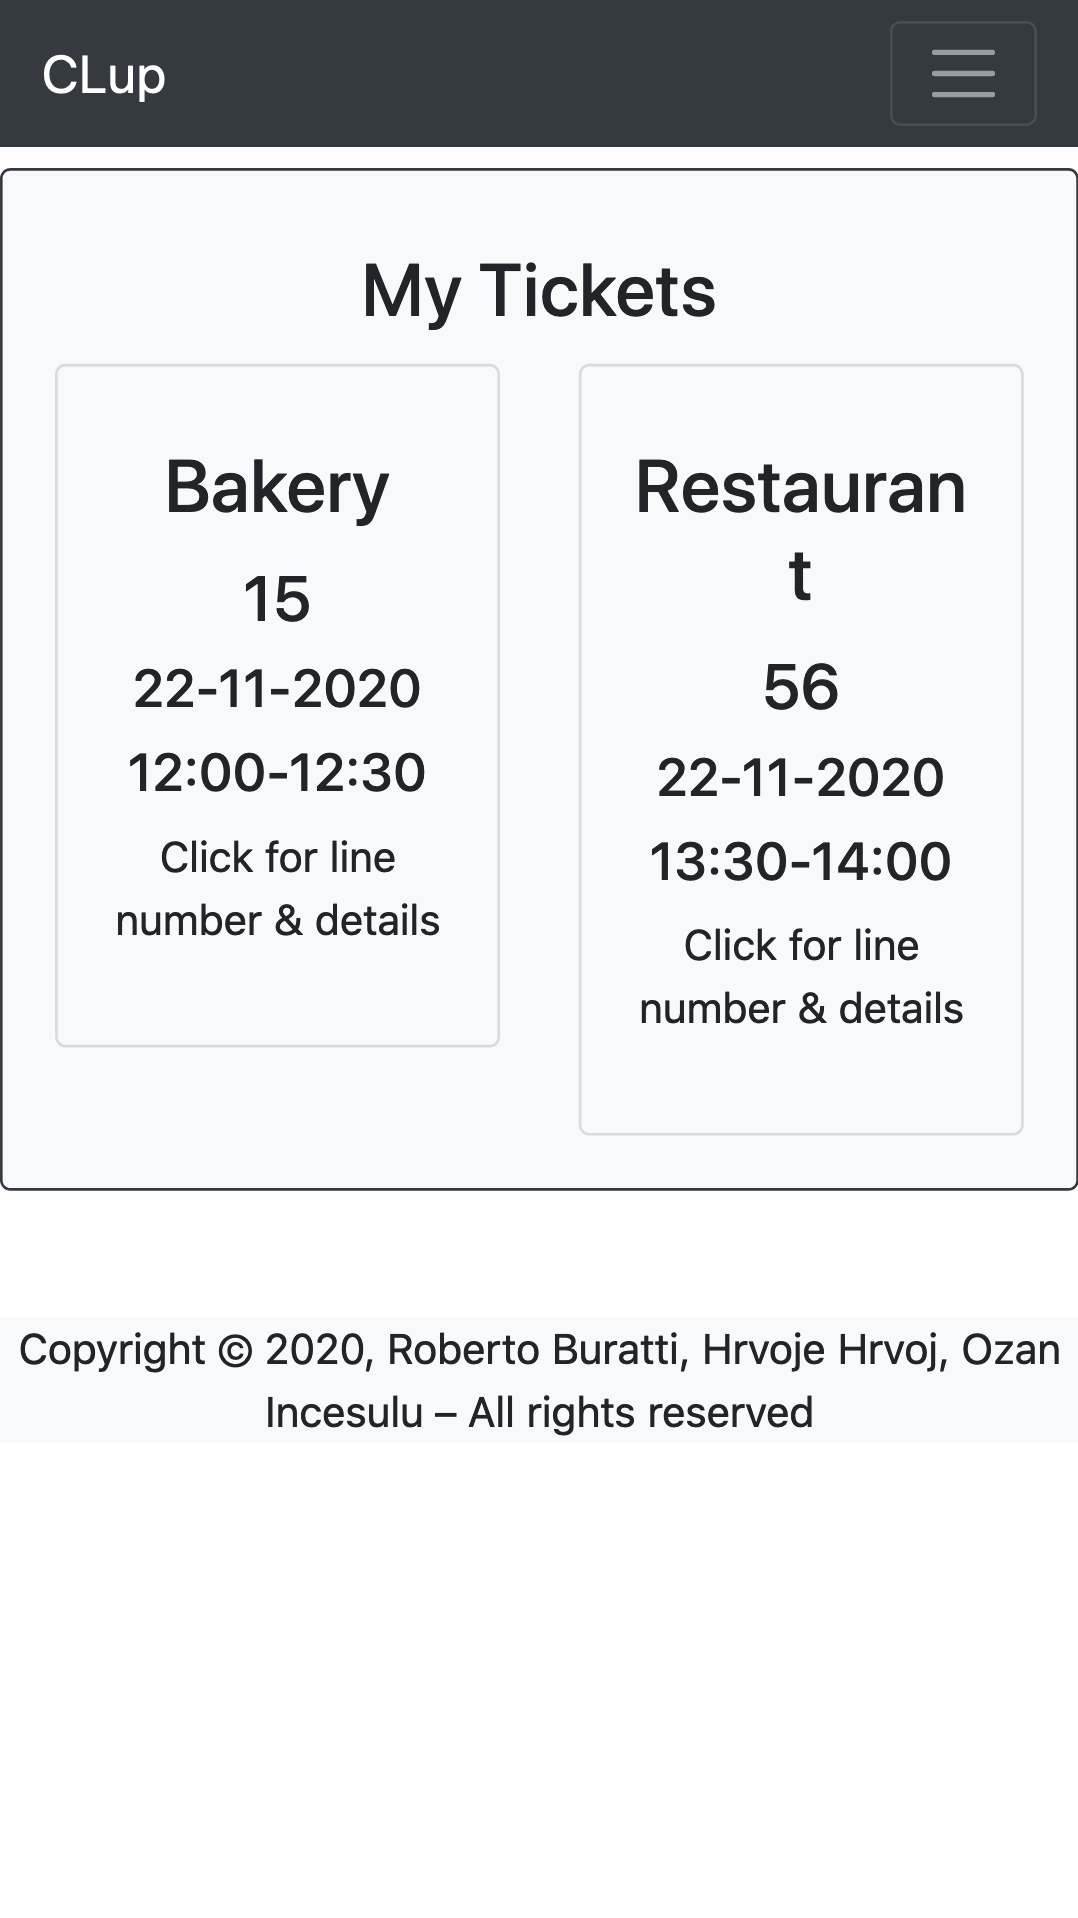
\includegraphics[width=0.9\textwidth]{Images/Screenshots/ticketList.png}
        \caption{Screenshot: List tickets}
    \end{minipage}\hfill
    \begin{minipage}{0.45\textwidth}
        \centering
        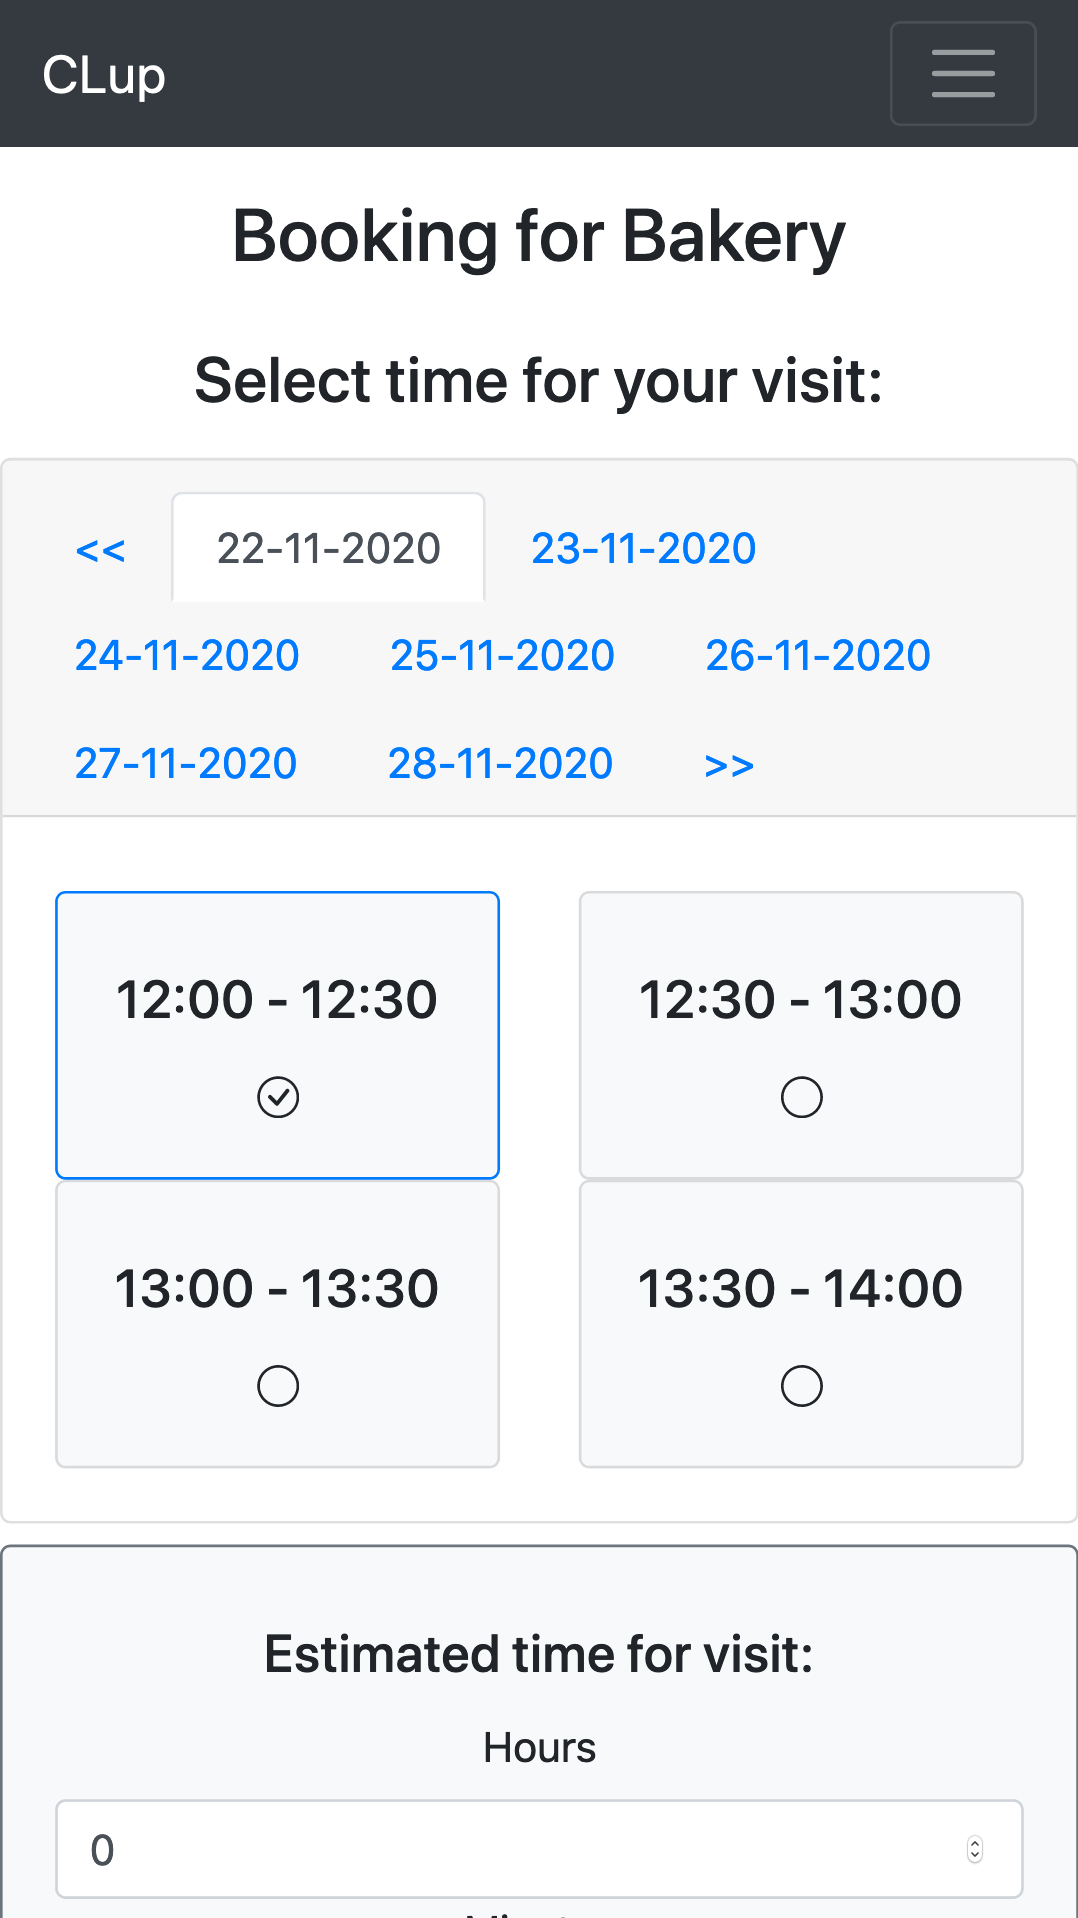
\includegraphics[width=0.9\textwidth]{Images/Screenshots/booking.png} % second figure itself
        \caption{Screenshot: Booking a new ticket}
    \end{minipage}
\end{figure}

\begin{figure}[H]
    \centering
    \begin{minipage}{0.45\textwidth}
        \centering
        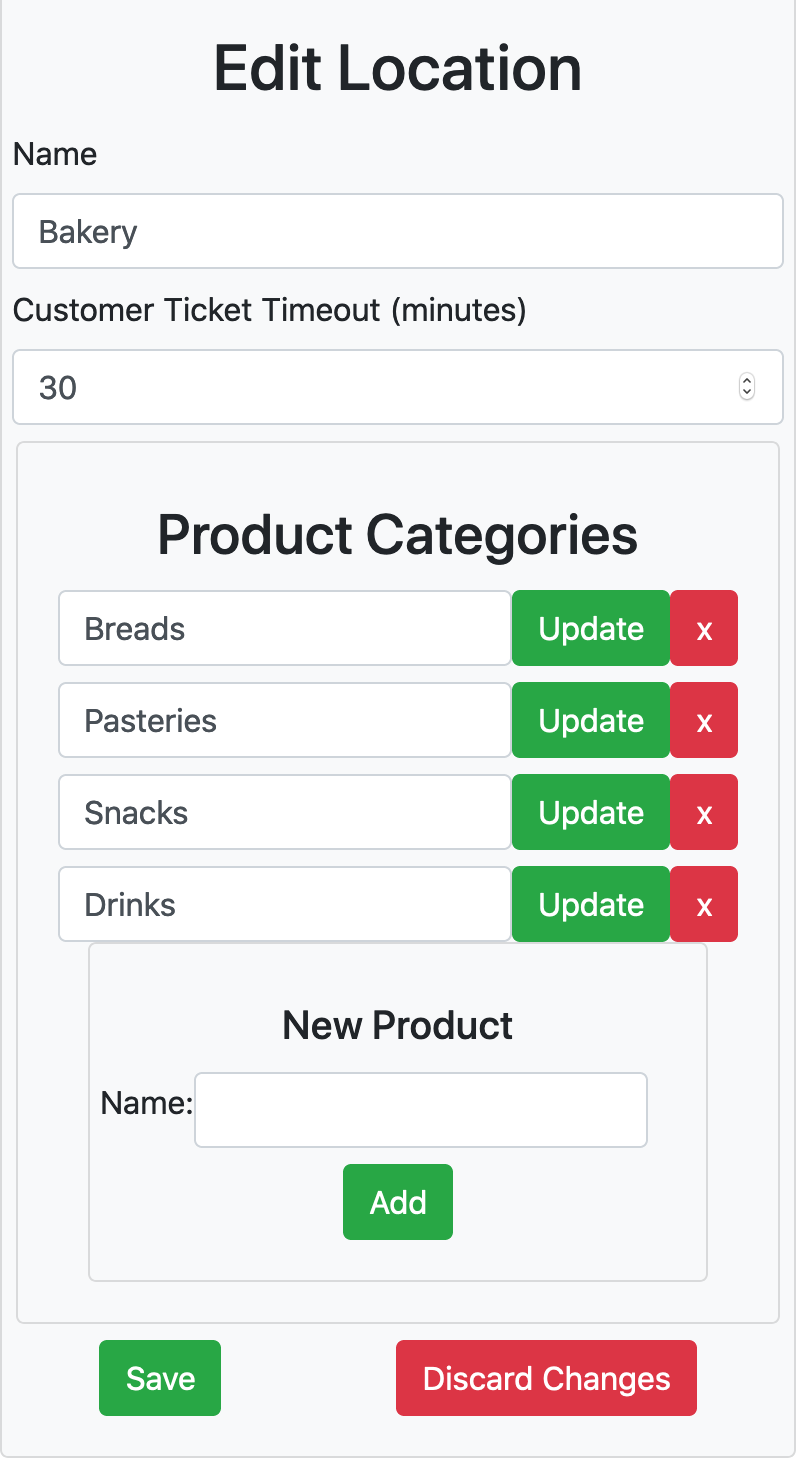
\includegraphics[width=0.9\textwidth]{Images/Screenshots/editLocation.png}
        \caption{Screenshot: Edit location screen of manager}
    \end{minipage}\hfill
    \begin{minipage}{0.45\textwidth}
        \centering
        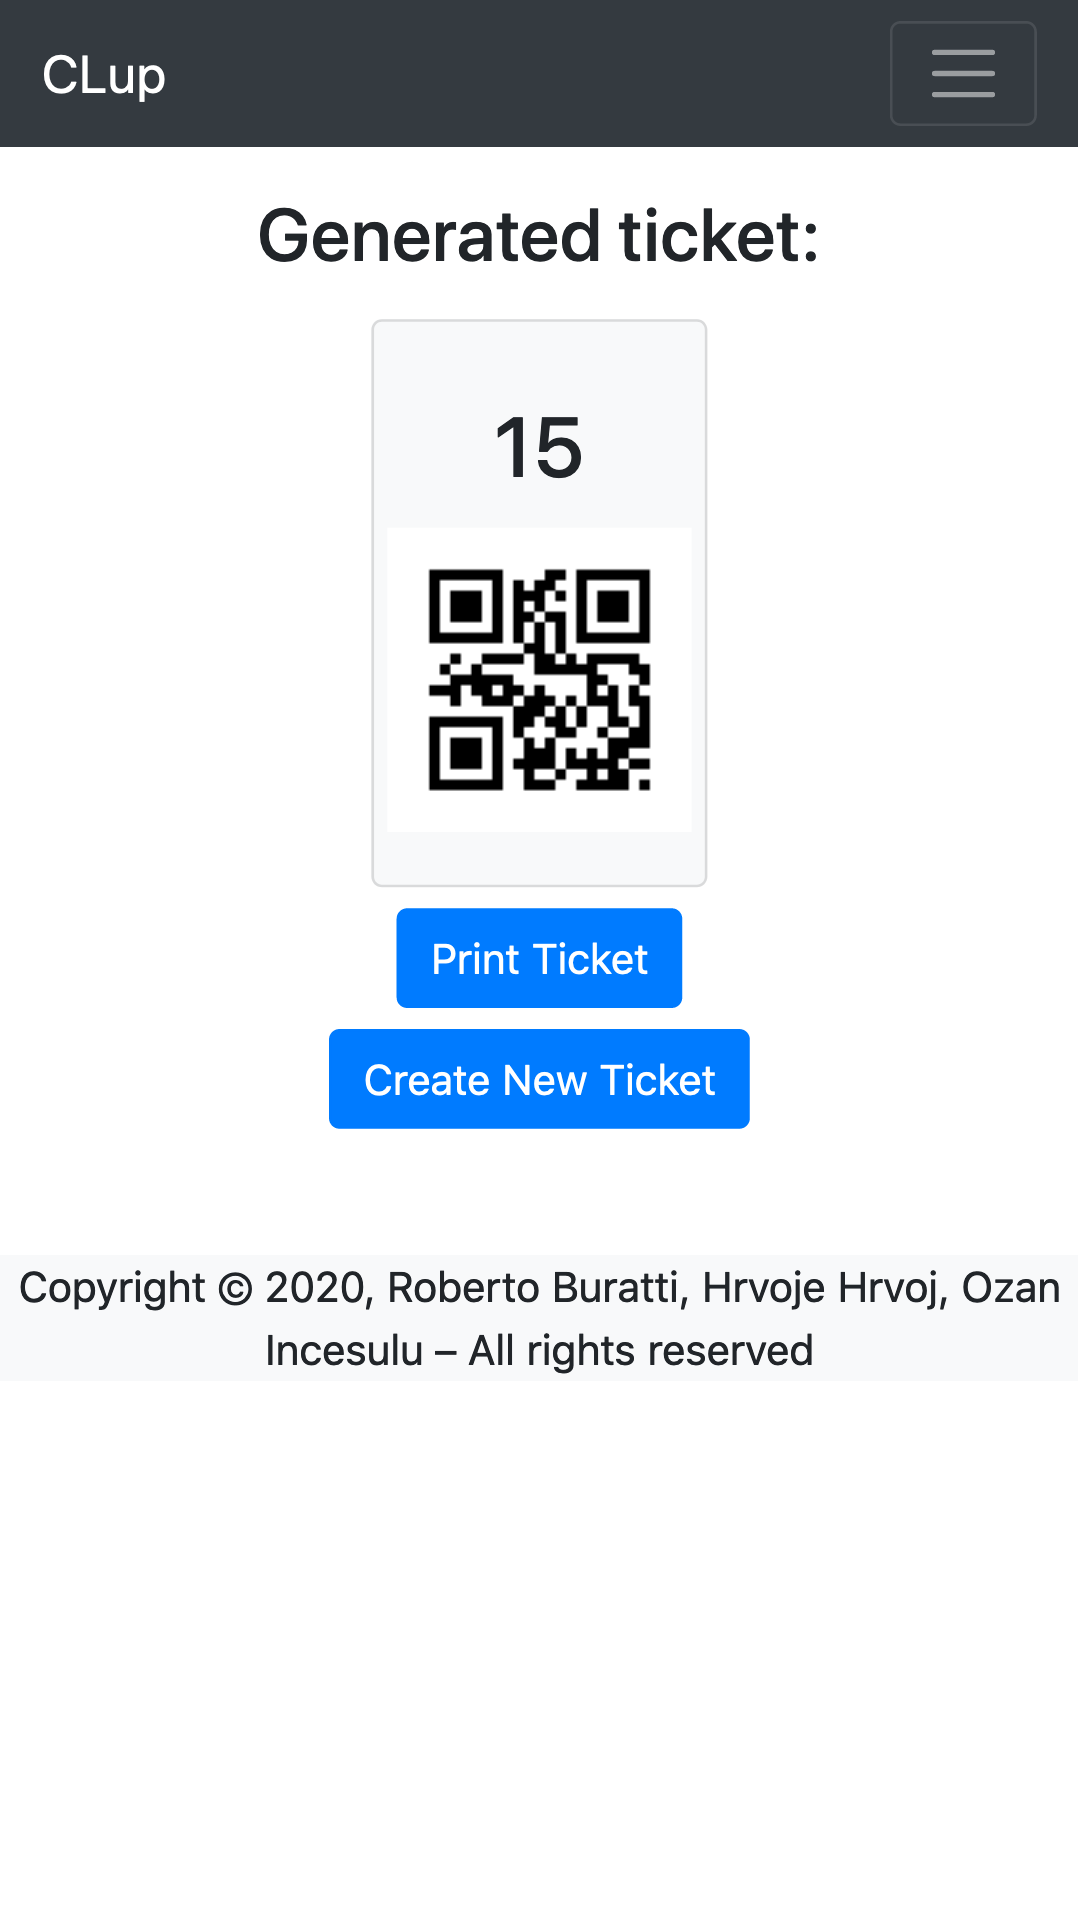
\includegraphics[width=0.9\textwidth]{Images/Screenshots/ticketGenerate.png} % second figure itself
        \caption{Screenshot: Ticket generate screen of clerk}
    \end{minipage}
\end{figure}

\begin{figure}[H]
    \centering
    \begin{minipage}{0.45\textwidth}
        \centering
        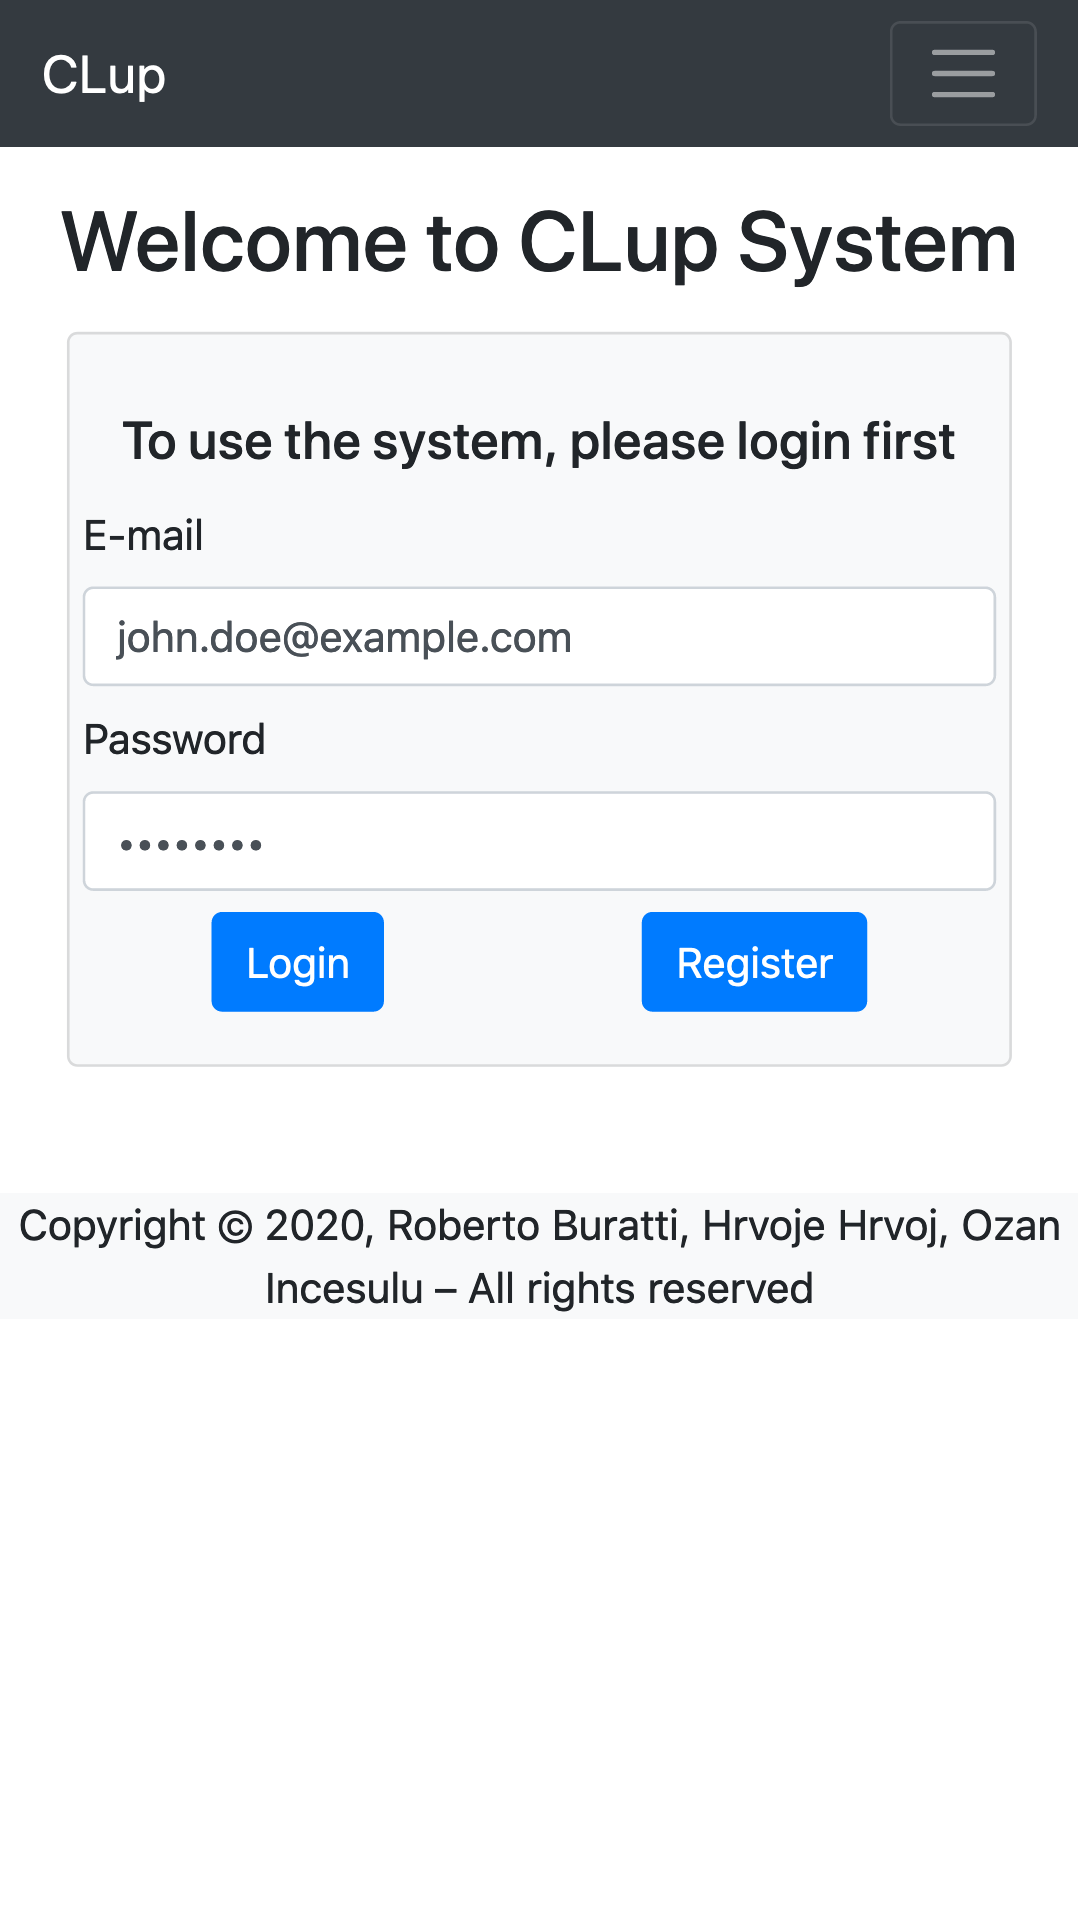
\includegraphics[width=0.9\textwidth]{Images/Screenshots/login.png}
        \caption{Screenshot: Login screen}
    \end{minipage}\hfill
    \begin{minipage}{0.45\textwidth}
        \centering
        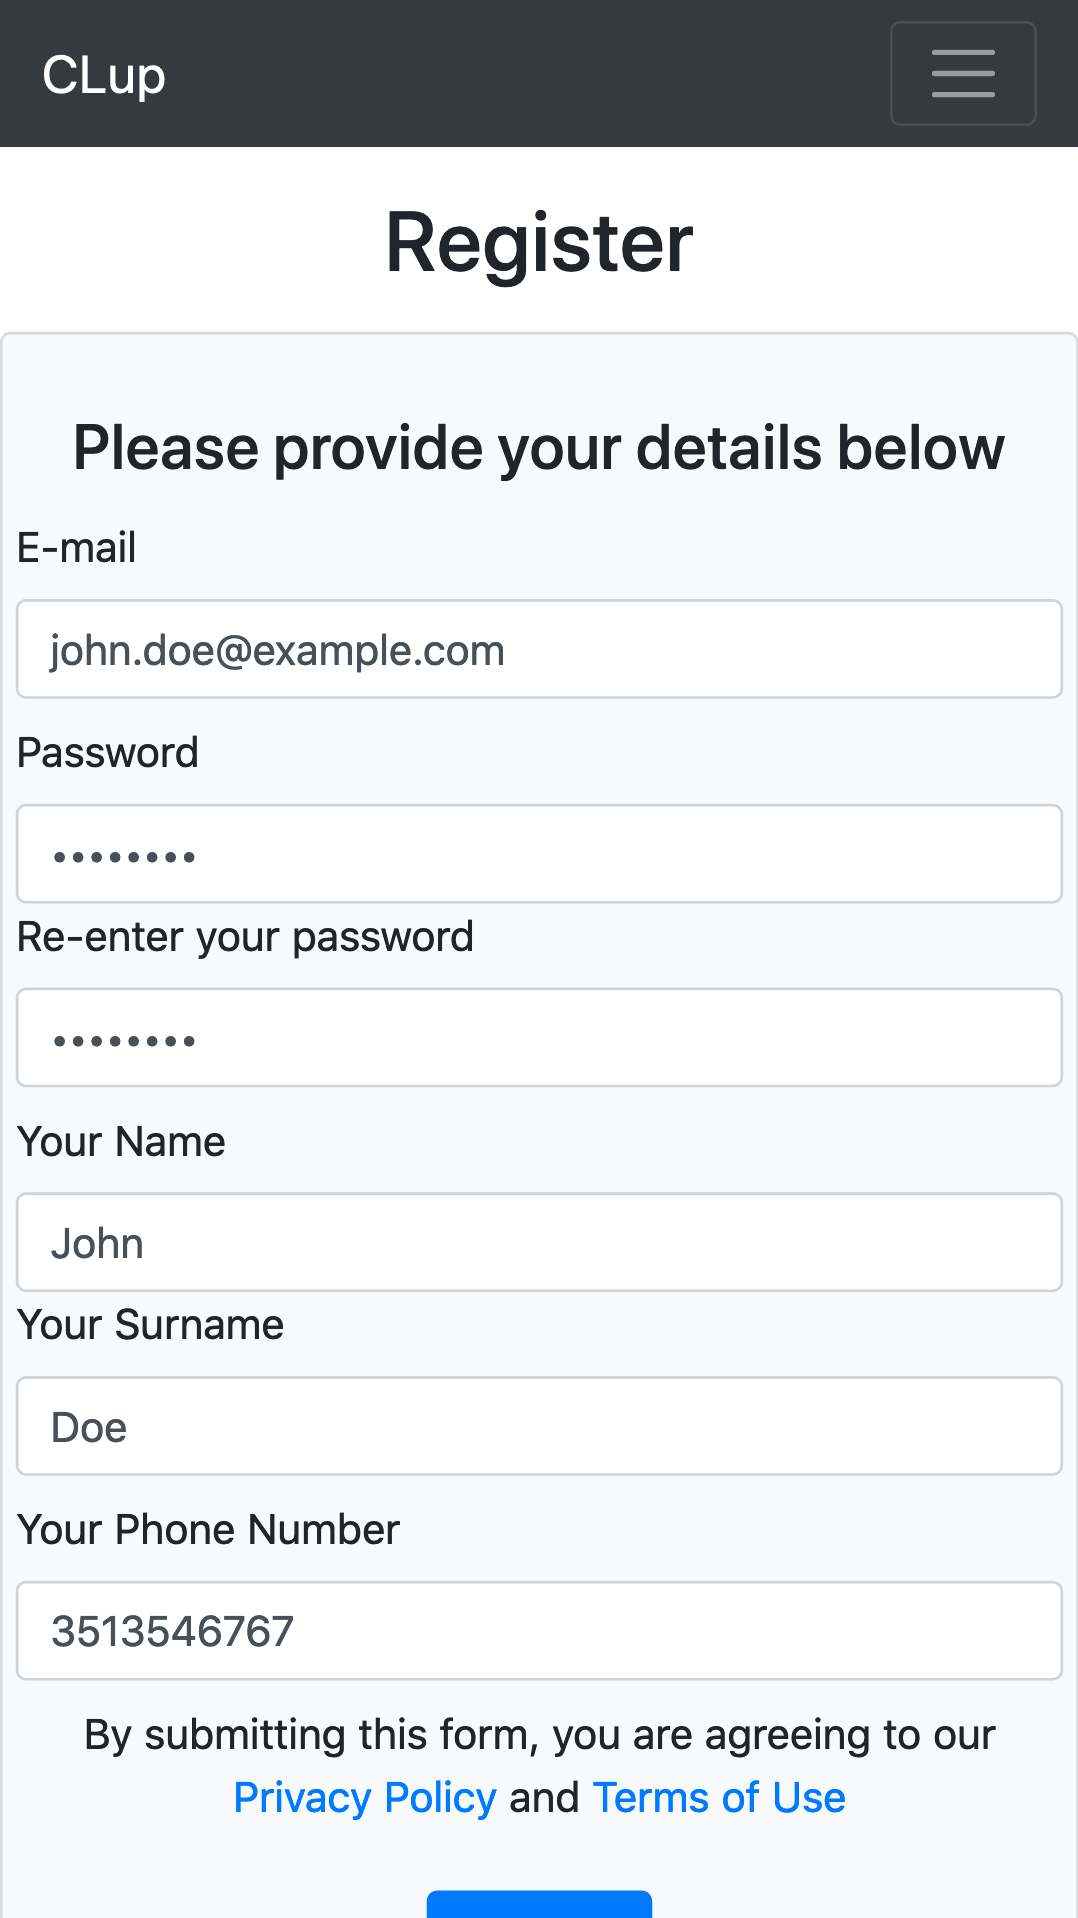
\includegraphics[width=0.9\textwidth]{Images/Screenshots/register.png} % second figure itself
        \caption{Screenshot: Register screen}
    \end{minipage}
\end{figure}
% Actual mockups of user interfaces

\subsubsection{Hardware Interfaces}
% TODO: @Hrvoje These 3
% Do we integrate with external hardware?
\subsubsection{Software Interfaces}

% Do we integrate with custom software, expose an API?

\subsubsection{Communication Interfaces}


% What is a communication interface? the Internet? RF port? Radio? Bluetooth?

\subsection{Functional Requirements}
% Use draw.io, compatible with GitHub.

% TODO: @Roberto finish the table and sequence diagrams
% Definition  of  use  case  diagrams,  use  cases  and  associated sequence/activity diagrams, and mapping on requirements

% Use case diagram

% For each use case:
%   Use case table
%   Use case sequence diagram
\subsubsection{Customer}

\begin{figure}[H]
    \centering
    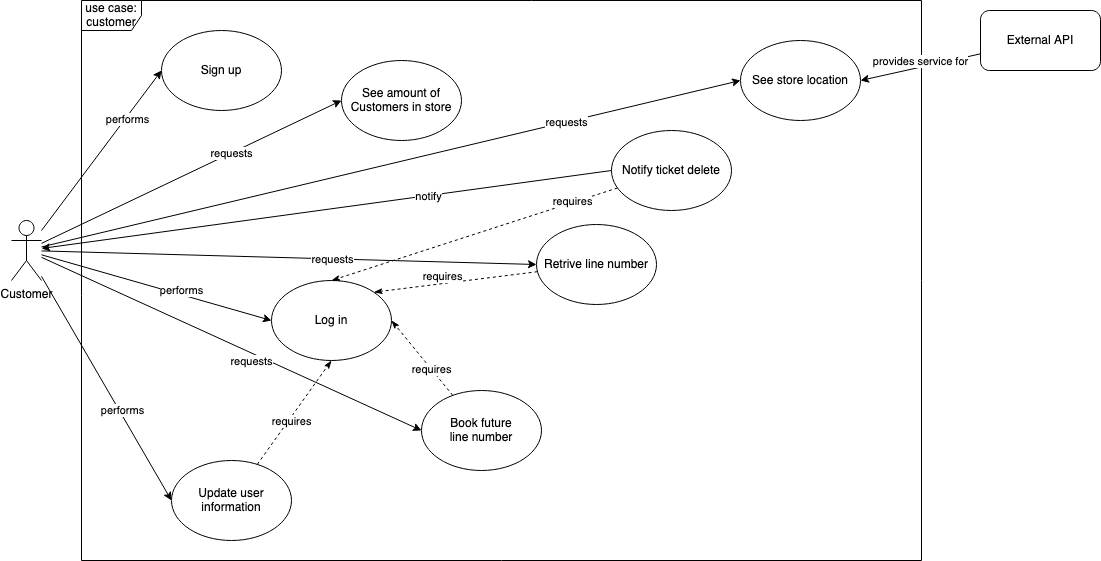
\includegraphics[height=0.5\textwidth]{Images/UseCaseDiagrams/Customer.png}
    \caption{Use Case Diagram for Customer}
\end{figure}
\textbf{Use cases}
\begin{table}[H]
    \begin{tabular}{|p{8cm}|p{8cm}|}
        \hline
        \textit{Name}    & \textbf{Book future line number} \\ \hline
        \textit{Actors} & Customer \\ \hline
        \textit{Entry conditions} & The customer is logged in the app and wants to book a visit to the store. \\ \hline
        \textit{Event flows}      & \tabitem The customer clicks on the "Book a Visit" button in the app. \\
        & \tabitem The app asks the time slot and the estimated time of the visit presenting as default value the average of the previous times of visit of the same user. \\
        & \tabitem The customer sets the time slot and the estimated time of their visit. \\
        & \tabitem The app asks what category of products the customer wants to buy. \\
        & \tabitem The customer set the products categories. \\
        & \tabitem The app requests the line number from the server. \\
        & \tabitem The app generates the QR code on the response from the server. \\
        \hline
        \textit{Exit conditions} & The customer has booked a visit for the store. \\ \hline
        \textit{Exceptions} & \tabitem The server cannot retrieve the line number since the time slot is full.\\ \hline
    \end{tabular}
    \caption{Use Case: Book future line number}
\end{table}
\begin{figure}[H]
    \centering
    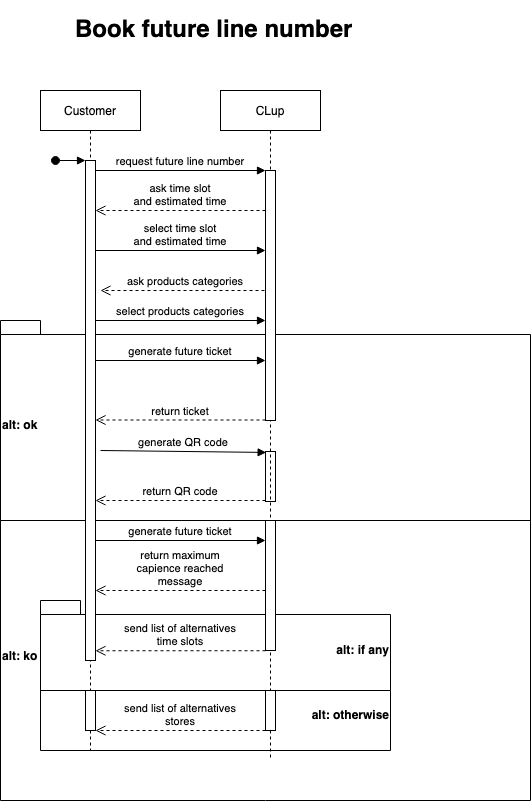
\includegraphics[height=0.5\textwidth]{Images/SequenceDiagrams/Customer/BookFutureLineNumberUseCaseSequenceDiagram.png}
    \caption{Sequence Diagram for Use Case: Book future line number}
\end{figure}
\begin{table}[H]
    \begin{tabular}{|p{8cm}|p{8cm}|}
        \hline
        \textit{Name}    & \textbf{See amount of customers in the store} \\ \hline
        \textit{Actors} & Customer \\ \hline
        \textit{Entry conditions} & The customer is logged in the app and wants to know how many customers are in the store in order to decide whether to book a visit or retrieve a line number \\ \hline
        \textit{Event flows}      & \tabitem The customer clicks on the  "Live Store Info" button. \\
        & \tabitem The app sends a count request to the server. \\
        & \tabitem The server returns the live data for the amount of customers in the store for each time slot. \\
        \hline
        \textit{Exit conditions} & The customer knows the amount of customers in the store and can plan their visit. \\ \hline
        \textit{Exceptions} & \\ \hline
    \end{tabular}
    \caption{Use Case: See amount of customers in the store}
\end{table}
\begin{figure}[H]
    \centering
    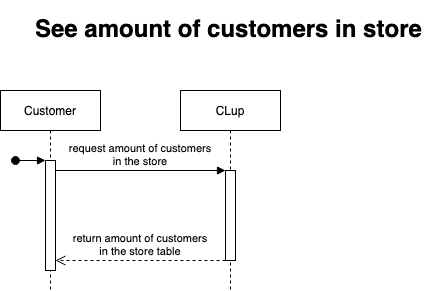
\includegraphics[height=0.5\textwidth]{Images/SequenceDiagrams/Customer/SeeAmountOfCustomersInStoreUseCaseSequenceDiagram.png}
    \caption{Sequence Diagram for Use Case: See amount of customers in the store}
\end{figure}
\begin{table}[H]
    \begin{tabular}{|p{8cm}|p{8cm}|}
        \hline
        \textit{Name}    & \textbf{See store location} \\ \hline
        \textit{Actors} & Customer, Maps API \\ \hline
        \textit{Entry conditions} & The customer needs to know where the store is located and the travel time \\ \hline
        % TODO: Are entry conditions things already met (user logged in) or intention (Customer wants, needs etc...)
        \textit{Event flows}      & \tabitem The customer clicks on the "Store Location" button. \\
        & \tabitem The app contacts the Maps API with the store location. \\
        & \tabitem The Maps API returns a map from the customer position to the store with a time estimation. \\
        \hline
        \textit{Exit conditions} & The customer knows how to go to the store and the travel time needed. \\ \hline
        \textit{Exceptions} & \tabitem The customer's smartphone doesn't provide or allow access to location services. \\
        \hline
    \end{tabular}
    \caption{Use Case: See store location}
\end{table}
\begin{figure}[H]
    \centering
    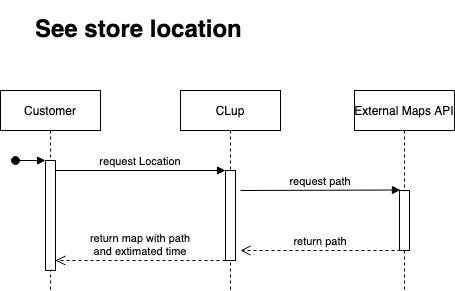
\includegraphics[height=0.5\textwidth]{Images/SequenceDiagrams/Customer/SeeStoreLocationUseCaseSequenceDiagram.png}
    \caption{Sequence Diagram for Use Case: See store location}
\end{figure}
\begin{table}[H]
    \begin{tabular}{|p{8cm}|p{8cm}|}
        \hline
        \textit{Name}    & \textbf{Sign up} \\ \hline
        \textit{Actors} & Customer \\ \hline
        \textit{Entry conditions} & The customer opened the app and they are not registered yet, and they want to register. \\ \hline
        \textit{Event flows}      & \tabitem The customer clicks on the "Sign Up" button. \\
        & \tabitem The customer inserts their credentials. \\
        & \tabitem The app sends the information to the server. \\
        & \tabitem The server stores the data related to the user. \\
        & \tabitem The server returns an acknowledgement to the app. \\
        \hline
        \textit{Exit conditions} & The customer is now registered and can use all the functionalities of the app. \\ \hline
        \textit{Exceptions} & \tabitem The e-mail provided in the registration form is already used by another user. \\
        & \tabitem The credentials provided in the registration form are ill-formatted.\\
        \hline
    \end{tabular}
    \caption{Use Case: Sign up}
\end{table}
\begin{figure}[H]
    \centering
    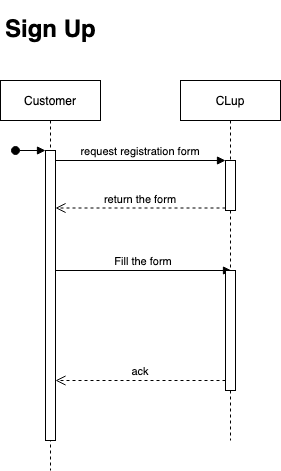
\includegraphics[height=0.5\textwidth]{Images/SequenceDiagrams/Customer/SignUpUseCaseSequenceDiagram.png}
    \caption{Sequence Diagram for Use Case: Sign up}
\end{figure}
\begin{table}[H]
    \begin{tabular}{|p{8cm}|p{8cm}|}
        \hline
        \textit{Name}    & \textbf{Login} \\ \hline
        \textit{Actors} & User \\ \hline
        \textit{Entry conditions} & The user has already sign up and wants to login to use CLup functionalities \\ \hline
        \textit{Event flows}     & \tabitem The customer clicks on the "Login" button\\
        & \tabitem The user provides their login credentials. \\
        & \tabitem The system authenticates the user \\
        \hline
        \textit{Exit conditions} & The user is logged in and can now use all the CLup functionalities \\ \hline
        \textit{Exceptions} & \tabitem The credentials are wrong \\
        \hline
    \end{tabular}
    \caption{Use Case: Login}
\end{table}
\begin{figure}[H]
    \centering
    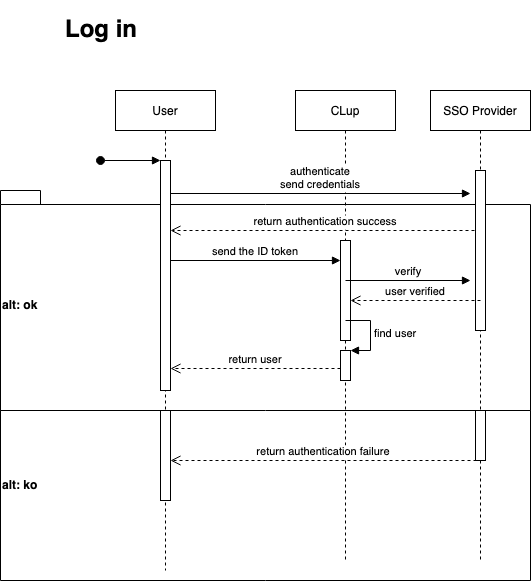
\includegraphics[height=0.5\textwidth]{Images/SequenceDiagrams/LogInUseCaseSequenceDiagram.png}
    \caption{Sequence Diagram for Use Case: Login}
\end{figure}
\begin{table}[H]
    \begin{tabular}{|p{8cm}|p{8cm}|}
        \hline
        \textit{Name}    & \textbf{Notify ticket delete} \\ \hline
        \textit{Actors} & Customer \\ \hline
        \textit{Entry conditions} & A ticket of the Customer was deleted from the server. \\ \hline
        \textit{Event flows}     & \tabitem The system sends an email to the customer to notify the deletion of their ticket\\
        \hline
        \textit{Exit conditions} & The customer is informed about the deletion of their ticket. \\ \hline
        \textit{Exceptions} & \tabitem \\
        \hline
    \end{tabular}
    \caption{Use Case: Notify ticket delete}
\end{table}
\begin{figure}[H]
    \centering
    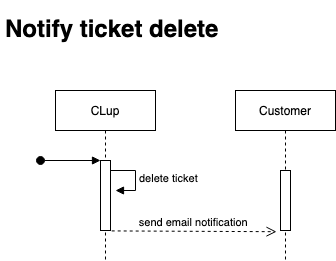
\includegraphics[height=0.5\textwidth]{Images/SequenceDiagrams/Customer/NotifyTicketDeleteUseCaseSequenceDiagram.png}
    \caption{Sequence Diagram for Use Case: Notify ticket delete}
\end{figure}
\begin{table}[H]
    \begin{tabular}{|p{8cm}|p{8cm}|}
        \hline
        \textit{Name}    & \textbf{Update user information} \\ \hline
        \textit{Actors} & User \\ \hline
        \textit{Entry conditions} & The user wants to change an information of themselves. \\ \hline
        \textit{Event flows}     & \tabitem The user clicks on the "Update User Information" button. \\
        & \tabitem The app shows a form precompiled with user's previous information. \\
        & \tabitem The user changes the information on the respective fields and presses the "Submit" button. \\
        & \tabitem The system saves the changes. \\
        \hline
        \textit{Exit conditions} & The user successfully updated their information. \\ \hline
        \textit{Exceptions} & \tabitem The new information provided is ill-formatted. \\
        \hline
    \end{tabular}
    \caption{Use Case: Update user information}
\end{table}
\begin{figure}[H]
    \centering
    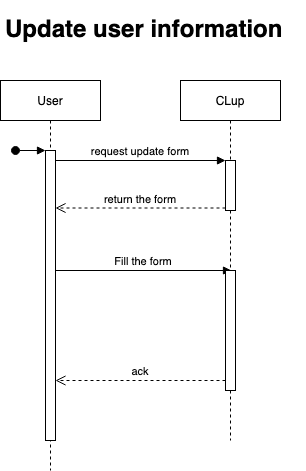
\includegraphics[height=0.5\textwidth]{Images/SequenceDiagrams/UpdateUserInformationUseCaseSequenceDiagram.png}
    \caption{Sequence Diagram for Use Case: Update user information}
\end{figure}

\subsubsection{Clerk}

\begin{figure}[H]
    \centering
    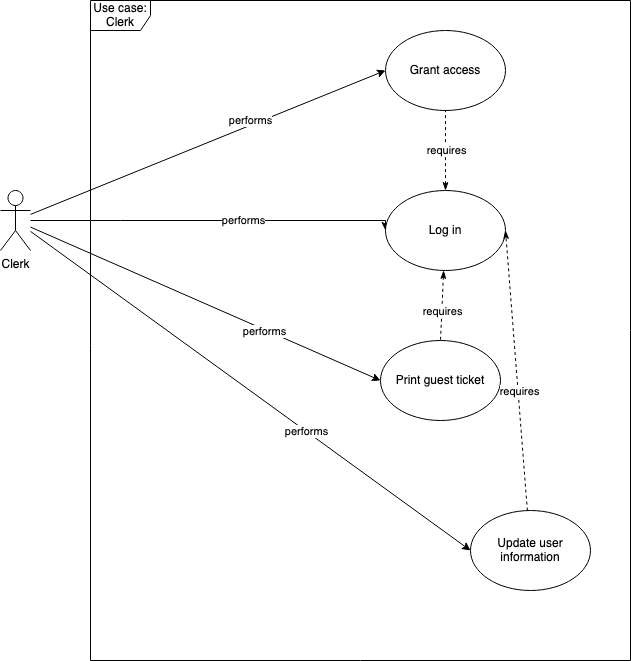
\includegraphics[height=0.5\textwidth]{Images/UseCaseDiagrams/Clerk.png}
    \caption{Use Case Diagram for Clerk}
\end{figure}

\textbf{Use cases}

\begin{table}[H]
    \begin{tabular}{|p{8cm}|p{8cm}|}
        \hline
        \textit{Name}    & \textbf{Grant access} \\ \hline
        \textit{Actors} & Clerk, Customer \\ \hline
        \textit{Entry conditions} & The customer has already obtained the QR code and they plan on entering the store.\\ \hline
        \textit{Event flows}      & \tabitem The Clerk scans the QR code from the customer's smartphone or printed ticket using the app \\
        & \tabitem The app analyzes the QR code and contacts to the Server \\
        & \tabitem The server decides if the customer can enter based on the information received in the QR code \\
        & \tabitem The server responds to the clerk app with the result \\
        & \tabitem The clerk let the customer enter the store \\ % TODO: Are we supposed to write about world phenomena?
        \\ \hline
        \textit{Exit conditions} & The customer enters the store \\ \hline
        \textit{Exceptions} & \tabitem The server communicates to the clerk that the customer cannot enter because their line number is not available.\\ \hline
    \end{tabular}
    \caption{Use Case: Grant access}
\end{table}
\begin{figure}[H]
    \centering
    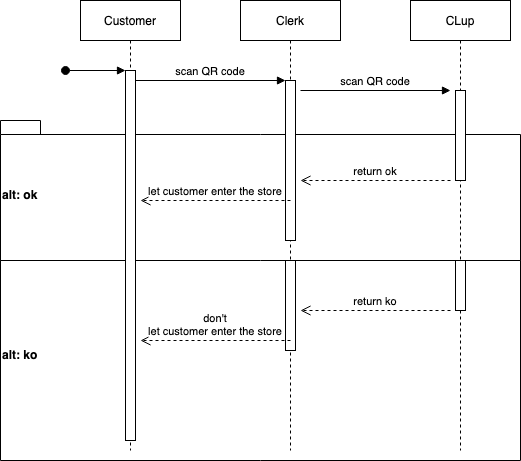
\includegraphics[height=0.5\textwidth]{Images/SequenceDiagrams/Clerk/GrantAccessUseCaseSequenceDiagram.png}
    \caption{Sequence Diagram for Use Case: Update user information}
\end{figure}
\begin{table}[H]
    \begin{tabular}{|p{8cm}|p{8cm}|}
        \hline
        \textit{Name}    & \textbf{Print guest ticket} \\ \hline
        \textit{Actors} & Clerk, Customer \\ \hline
        \textit{Entry conditions} & The customer has arrived to the location, doesn't have a ticket on their smartphone, and needs a physical ticket to enter. \\ \hline
        \textit{Event flows}      & \tabitem The customer asks the clerk for a ticket. \\
        & \tabitem The clerk generate a ticket using the app. \\
        & \tabitem The app sends a request to the server to generate a ticket. \\
        & \tabitem The server generates a line number and a ticket. \\
        & \tabitem The server sends the ticket back to the app. \\
        & \tabitem The clerk prints the ticket. \\ % TODO: Real world phenomena here again?
        & \tabitem The clerk gives the ticket to the customer. \\
        \hline
        \textit{Exit conditions} & The customer has a ticket. \\ \hline
        \textit{Exceptions} & \tabitem The server cannot generate a line number due to capacity constraints. \\ \hline
    \end{tabular}
    \caption{Use Case: Print guest ticket}
\end{table}
\begin{figure}[H]
    \centering
    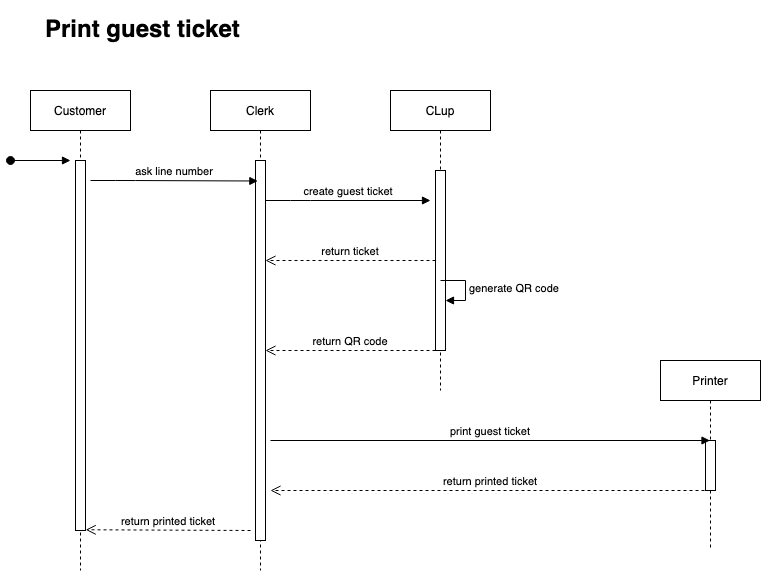
\includegraphics[height=0.5\textwidth]{Images/SequenceDiagrams/Clerk/PrintGuestTicketUseCaseSequenceDiagram.png}
    \caption{Sequence Diagram for Use Case: Print guest ticket}
\end{figure}

\subsubsection{Manager}

\begin{figure}[H]
    \centering
    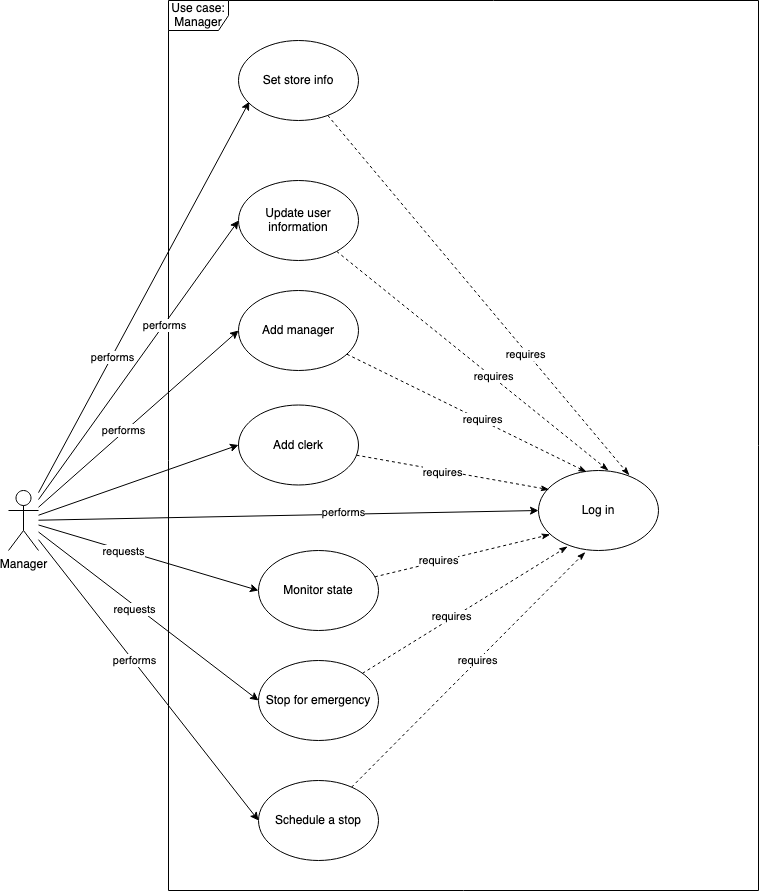
\includegraphics[height=0.5\textwidth]{Images/UseCaseDiagrams/Manager.png}
    \caption{Use Case Diagram for Manager}
\end{figure}

\textbf{Use cases}

\begin{table}[H]
    \begin{tabular}{|p{8cm}|p{8cm}|}
        \hline
        \textit{Name}    & \textbf{Initialize} \\ \hline
        \textit{Actors} & Manager \\ \hline
        \textit{Entry conditions} & The manager of the store needs to set the basic information of the store in order to start the service \\ \hline
        \textit{Event flows}      & \tabitem The manager clicks on the initialize button \\
        & \tabitem The app shows the location form to the manager \\
        & \tabitem The manager fills the form and sends ıt to the server via the app\\
        & \tabitem The server registers the information and acknowledges \\
        \hline
        \textit{Exit conditions} & The system is initialized and can offer all its functions \\ \hline
        \textit{Exceptions} & \tabitem Some mandatory parts of the form are not filled. \\ \hline
    \end{tabular}
    \caption{Use Case: Initialize}
\end{table}

% TODO: There is no request for info form, front-end is capable of generating such info.
\begin{figure}[!htbp]
    \centering
    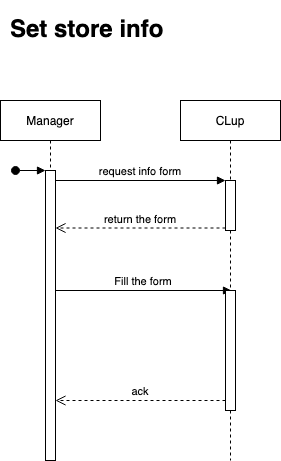
\includegraphics[height=0.5\textwidth]{Images/SequenceDiagrams/Manager/SetStoreInfoUseCaseSequenceDiagram.png}
    \caption{Sequence Diagram for Use Case: Initialize}
\end{figure}
\begin{table}[H]
    \begin{tabular}{|p{8cm}|p{8cm}|}
        \hline
        \textit{Name}    & \textbf{Monitor state} \\ \hline
        \textit{Actors} & Manager \\ \hline
        \textit{Entry conditions} & The manager wants to monitor the number of customers in the store in real time. \\ \hline
        \textit{Event flows}      & \tabitem The manager clicks on the "Monitoring" button. \\
        & \tabitem The app sends the number request to the server.  \\
        & \tabitem The server returns the number of customers in the store. \\
        & \tabitem The app repeats the process periodically as long as the monitoring page is open. \\ % TODO: What period? Do we need to specify this?
        \hline
        \textit{Exit conditions} & The manager is informed on the number of the customers in the store in real time. \\ \hline
        \textit{Exceptions} & \tabitem \\ \hline
    \end{tabular}
    \caption{Use Case: Monitor state}
\end{table}
\begin{figure}[H]
    \centering
    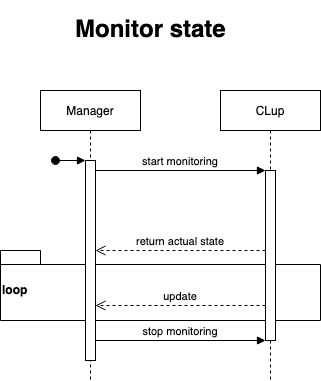
\includegraphics[height=0.5\textwidth]{Images/SequenceDiagrams/Manager/MonitorStateUseCaseSequenceDiagram.png}
    \caption{Sequence Diagram for Use Case: Monitor state}
\end{figure}
\begin{table}[H]
    \begin{tabular}{|p{8cm}|p{8cm}|}
        \hline
        \textit{Name}    & \textbf{Schedule a stop} \\ \hline
        \textit{Actors} & Manager \\ \hline
        \textit{Entry conditions} & The manager wants to schedule a period of time in which the store will be closed so the users can not book a visit for that time. \\ \hline
        \textit{Event flows}      & \tabitem The manager clicks on the "Schedule a Stop" button. \\
        & \tabitem The app shows a form for the time of the stop. \\
        & \tabitem The manager fills the form and submits it to the server through the app. \\
        & \tabitem The server stores the information in the database and returns an acknowledgement. \\
        \hline
        \textit{Exit conditions} & The system has a scheduled stop stored in its database and will use it to prevent customers from booking a visit in that time period. \\ \hline
        \textit{Exceptions} & \tabitem There is already a planned stop in that period. \\ \hline
    \end{tabular}
    \caption{Use Case: Schedule a stop}
\end{table}
\begin{figure}[H]
    \centering
    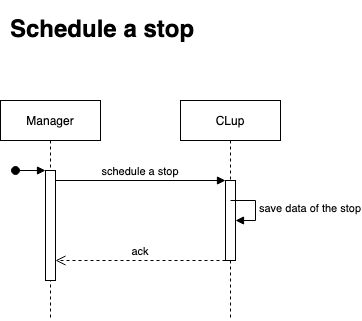
\includegraphics[height=0.5\textwidth]{Images/SequenceDiagrams/Manager/ScheduleAStopUseCaseSequenceDiagram.png}
    \caption{Sequence Diagram for Use Case: Schedule a stop}
\end{figure}
\begin{table}[H]
    \begin{tabular}{|p{8cm}|p{8cm}|}
        \hline
        \textit{Name}    & \textbf{Stop for emergency} \\ \hline
        \textit{Actors} & Manager \\ \hline
        \textit{Entry conditions} & An emergency occurred and the manager wants to immediately stop the system from distributing line numbers. \\ \hline
        \textit{Event flows}     & \tabitem The manager click on the "Emergency Stop" button \\
        & \tabitem The app asks for confirmation from the manager. \\
        & \tabitem The manager confirms the stop of the system. \\
        & \tabitem The app sends the system stop request to the server. \\
        & \tabitem The server stops the service and return an acknowledgement. \\
        \hline
        \textit{Exit conditions} & The system has interrupted the service. \\ \hline
        \textit{Exceptions} & \tabitem The manager aborts the operation. \\
        \hline
    \end{tabular}
    \caption{Use Case: Stop for emergency}
\end{table}
\begin{figure}[H]
    \centering
    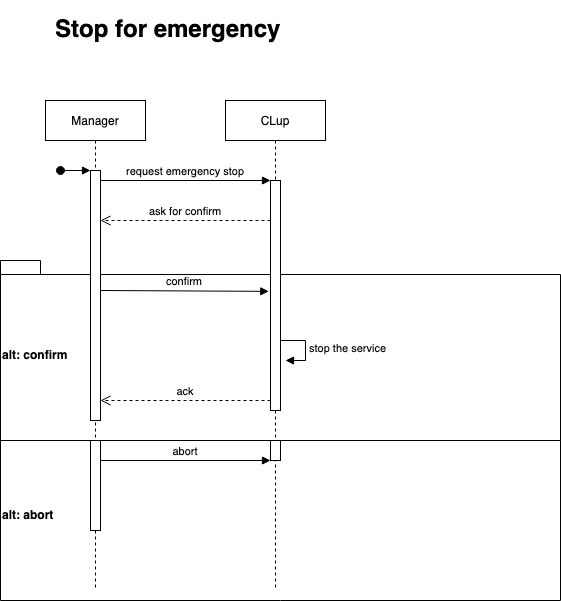
\includegraphics[height=0.5\textwidth]{Images/SequenceDiagrams/Manager/StopForEmergencyUseCaseSequenceDiagram.png}
    \caption{Sequence Diagram for Use Case: Stop for emergency}
\end{figure}
\begin{table}[H]
    \begin{tabular}{|p{8cm}|p{8cm}|}
        \hline
        \textit{Name}    & \textbf{Add Clerk} \\ \hline
        \textit{Actors} & Manager \\ \hline
        \textit{Entry conditions} & The manager wants to add a new clerk to the system \\ \hline
        \textit{Event flows}     & \tabitem The manager click on the "add clerk" button \\
        & \tabitem The system asks the data of the new clerk (e.g. the credentials) \\
        & \tabitem The manager inserts the data and press "submit" \\
        \hline
        \textit{Exit conditions} & The new clerk is added to the system \\ \hline
        \textit{Exceptions} & \tabitem The data of the clerk are incomplete or incorrect \\
        \hline
    \end{tabular}
    \caption{Use Case: Add Clerk}
\end{table}
\begin{figure}[H]
    \centering
    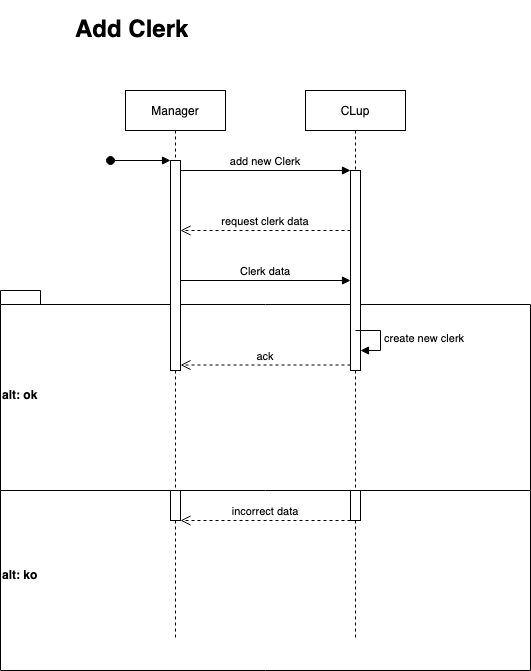
\includegraphics[height=0.5\textwidth]{Images/SequenceDiagrams/Manager/AddClerkUseCaseSequenceDiagram.png}
    \caption{Sequence Diagram for Use Case: Add Clerk}
\end{figure}
\begin{table}[H]
    \begin{tabular}{|p{8cm}|p{8cm}|}
        \hline
        \textit{Name}    & \textbf{Add Manager} \\ \hline
        \textit{Actors} & Manager \\ \hline
        \textit{Entry conditions} & The manager wants to add a new manager to the system \\ \hline
        \textit{Event flows}     & \tabitem The manager click on the "Add Manager" button \\
        & \tabitem The system asks the data of the new manager (e.g. the credentials) \\
        & \tabitem The manager inserts the data and press "Submit" \\
        \hline
        \textit{Exit conditions} & The new Manager is added to the system \\ \hline
        \textit{Exceptions} & \tabitem The data of the Manager are incomplete or incorrect \\
        \hline
    \end{tabular}
    \caption{Use Case: Add Manager}
\end{table}
\begin{figure}[H]
    \centering
    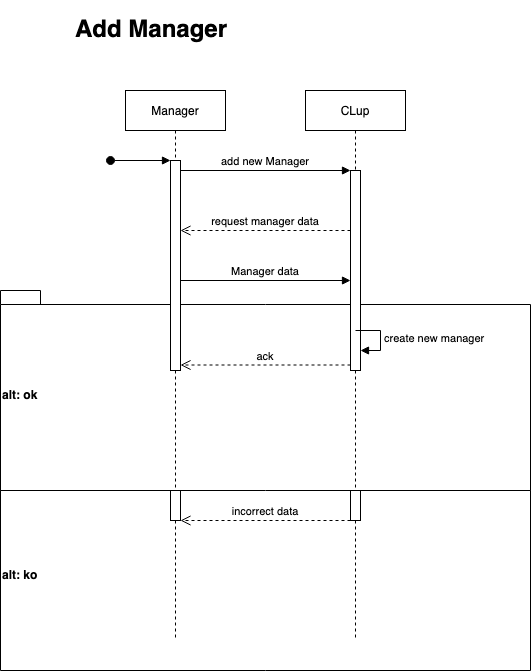
\includegraphics[height=0.5\textwidth]{Images/SequenceDiagrams/Manager/AddManagerUseCaseSequenceDiagram.png}
    \caption{Sequence Diagram for Use Case: Add Manager}
\end{figure}

\subsubsection{Requirements}
\begin{itemize}
    \item \textbf{$R_1$} The system must allow users to authenticate using their e-mail address and password.
    \item \textbf{$R_2$} The system must allow customers to register using their e-mail address, their name, surname, phone number and a new password.
    \item \textbf{$R_3$} The system must provide a hard-coded super user to allow addition of locations and managers of locations.
    \item \textbf{$R_4$} Managers must be able to add additional managers and clerks as users.
    \item \textbf{$R_5$} Managers must be able to set and update location specific information, that are maximum number of customers in the location at any given time, opening and closing hours of the store per each day, line number timeout, limit of reservation per customer on a predetermined time interval that is one of month, week or day, and location of the place % One form
    \item \textbf{$R_6$} Managers can add any other location as a partner store.
    \item \textbf{$R_7$} Managers can stop the system from issuing any more tickets for a given day
    \item \textbf{$R_8$} Managers can schedule the system stop for a future time.
    \item \textbf{$R_9$} Managers can set the in-shop locations for different categories and product items.
    \item \textbf{$R_{10}$} In case of a system stop, no further line numbers can be issued for the given time slots.
    \item \textbf{$R_{11}$} In case of a system stop, all line numbers in the stop time slots has to be cancelled.
    \item \textbf{$R_{12}$} The system must cancel those line numbers that the customer didn't arrive to the location for more than the set timeout interval.
    \item \textbf{$R_{13}$} In case of a ticket cancel, customer must be notified with an e-mail notification.
    \item \textbf{$R_{14}$} Clerks must register the entrance and exit of customers via scanning the QR code for their line number.
    \item \textbf{$R_{15}$} Clerks must be able to generate line number tickets in a printer compatible format.
    \item \textbf{$R_{17}$} Customers must be able to obtain a line number, except when the system is stopped or the store is full.
    \item \textbf{$R_{18}$} Customers must be able to obtain line numbers for different time slots in the future.
    \item \textbf{$R_{19}$} Customers can not obtain line numbers that exceed the quantity per time interval limits.
    \item \textbf{$R_{20}$} Customers can not obtain line numbers for time intervals that the system is stopped by a manager.
    \item \textbf{$R_{21}$} Customers must be able to see the estimated time available for their line number.
    \item \textbf{$R_{22}$} Customers must be able to set or update their phone number, password, name and surname.
    \item \textbf{$R_{23}$} Customers can select specific product and/or product categories they plan to visit in the location while obtaining a line number.
    \item \textbf{$R_{24}$} Customers can set an estimated time for their visit while obtaining a line number.
    \item \textbf{$R_{25}$} Customers must be able to view the shop location
    \item \textbf{$R_{26}$} Customers can view the occupation forecasts for the location at different time slots.
    \item \textbf{$R_{27}$} Customers can see the alternative suggestions for time slots while obtaining a line number for the future.
    \item \textbf{$R_{28}$} Customers can view the occupancy for the partner stores, if preferred time slot is not available while obtaining a line number.
    \item \textbf{$R_{29}$} Customers can view their line numbers with the number and the QR code.
    \item \textbf{$R_{30}$} The system must be able to provide a forecast for the occupancy of each location for any given time based on past visits.
\end{itemize}

% Goals, mapped to the requirements and domain assumptions they relate to
% (Requirements are vaguely given in Overview -> Product functions)
% (Domain assumptions are in Overview -> Assumptions,dependencies and constraints -> Domain Assumptions)


% TODO: Tracability Matrix, Summary table
\subsection{Performance Requirements}

% Some basic stuff about how much users the system takes, speed etc...

% TODO: @Hrvoje Complete these
\subsection{Design Constraints}

\subsubsection{Standards compliance}
% QR standard, UTC timing standard, GPS, etc...

\subsubsection{Hardware limitations}
% What needs to be on the phone?
\subsubsection{Any other constraint}
% GDPR regulations, local laws, etc...

% Isn't this similar to Overview -> Assumptions,dependencies and constraints -> Constraints?

\subsection{Software System Attributes}

\subsubsection{Reliability}

% Don't crash for long time, fault tolerance strategies like RAID, backups, etc

\subsubsection{Availability}

% 99.5% availability minimum, release any hardware control in case of power cut or unavailability.

\subsubsection{Security}

% Data hashing, salting, encryption of user data if necessary.

\subsubsection{Maintainability}

% Testing practices on all levels

\subsubsection{Portability}

% Usage of widely adopted platforms (Java, .NET, Browser), no custom protocol implementation apart from wide-spread


%------------------------------------------------------------------------------------------------------------------------------------------------
\clearpage
{\color{Blue}{\section{Formal Analysis Using Alloy}}}
\label{sect:alloy}
% This section should include a brief presentation of the main objectives driving the formal modeling activity,
% as well as a description of the model itself, what can be proved with it, and why what is proved is important
% given the problem at hand. To show the soundness and correctness of the model, this section can show some worlds
% obtained by running it, and/or the results of the checks performed on meaningful assertions.
% TODO: @Roberto: start
\subsection{Alloy introduction}

In this section is presented the Alloy representation of some critical
aspects the system must present. It is worth highlighting that below only
stable states are considered, in which the system may be found. As a
consequence, no edge cases are treated. \\
In particular, the following features are modelled:\\
- There can't never be more customers in a section then the maximum capacity of that section, in any given moment.\\
- A booking is possible only by a registered customer.\\
- Every visit to the store is granted by an access title.\\

\subsection{Alloy code}

\begin{lstlisting}
    //Signatures-------------------------------------------------------------------------------------------------------------------------

    abstract sig Store {
    sections : some Section
    }

    one sig PrimaryStore extends Store{
    partnerStores : set PartnerStore
    }

    sig PartnerStore extends Store {}

    sig Section {
    maxCapacity: one Int
    }{
    maxCapacity > 0
    }

    sig Email {}

    sig Password {}

    abstract sig User {
    email : one Email,
    password : one Password
    }

    sig Customer extends User {}

    some sig Manager extends User {
    store : one Store
    }

    some sig Clerk extends User {
    manager : one Manager,
    store : one Store
    }{
    manager.store = store
    }

    abstract sig AccessTitle{
    customer : lone Customer,
    sections: some Section,
    estimatedEnterTime : one Time,
    estimatedExitTime: one Time,
    }{
    estimatedEnterTime.timestamp < estimatedExitTime.timestamp

    }

    sig Ticket extends AccessTitle{
    lineNumber : one ActualLineNumber
    }

    sig Booking extends AccessTitle{
    lineNumber : one BookedLineNumber
    }{
    estimatedEnterTime.timestamp > lineNumber.timeSlot.start.timestamp
    estimatedEnterTime.timestamp < lineNumber.timeSlot.end.timestamp
    #customer = 1
    }

    sig Visit{
    accessTitle : one AccessTitle,
    enterTime : one Time,
    exitTime : lone Time
    }{
    enterTime.timestamp < exitTime.timestamp
    }

    //UTC standard format: number of seconds from 1970/01/01 00:00:00
    sig Time {
    timestamp : one Int
    }{
    timestamp>=0
    }

    sig TimeSlot {
    start : one Time,
    end : one Time
    }{
    start.timestamp < end.timestamp
    }

    abstract sig LineNumber {
    timeSlot : one TimeSlot,
    number : one Int
    }{
    number >= 0
    }

    sig ActualLineNumber extends LineNumber{}

    sig BookedLineNumber extends LineNumber{}

    //Facts-------------------------------------------------------------------------------------------------------------------------

    fact credentialInUsers {
    all mail : Email | mail in User.email
    all pw : Password | pw in User.password
    no mail : Email, disj user1, user2 : User | mail in user1.email && mail in user2.email
    no pw : Password, disj user1, user2 : User | pw in user1.password && pw in user2.password
    }

    fact everySectionInAStore {
    all section : Section | section in Store.sections
    no section : Section, disj store1, store2 : Store | section in store1.sections && section in store2.sections
    }

    fact everyLineNumberInAnAccessTitle {
    all ln : LineNumber | ln in (Ticket.lineNumber + Booking.lineNumber)
    no ln: LineNumber, disj t1, t2 : Ticket | ln in t1.lineNumber && ln in t2.lineNumber
    no ln: LineNumber, disj t1, t2 : Booking | ln in t1.lineNumber && ln in t2.lineNumber
    all disj ln1, ln2 :LineNumber | ln1.number = ln2.number => ln1.timeSlot != ln2.timeSlot
    }

    fact AVisitForEachAccessTitle {
    no at: AccessTitle, disj visit1, visit2 : Visit | at in visit1.accessTitle && at in visit2.accessTitle
    }

    fact everyPartnerSoreInAPrimaryStore {
    all partnerStore : PartnerStore | partnerStore in PrimaryStore.partnerStores
    }

    fact bookOnlyAStore {
    all accessTitle : AccessTitle | one store : Store | accessTitle.sections in store.sections
    }

    fact consistenQueue {
    all disj at1, at2 : AccessTitle |
    ((at1<:Ticket).lineNumber.number < (at2<:Ticket).lineNumber.number && (at1<:Ticket).lineNumber.timeSlot = (at2<:Ticket).lineNumber.timeSlot) =>
    at1.estimatedEnterTime.timestamp =< at2.estimatedEnterTime.timestamp

    all disj at1, at2 : AccessTitle |
    ((at1<:Booking).lineNumber.number < (at2<:Booking).lineNumber.number && (at1<:Booking).lineNumber.timeSlot = (at2<:Booking).lineNumber.timeSlot) =>
    at1.estimatedEnterTime.timestamp =< at2.estimatedEnterTime.timestamp
    }

    fact noOverBooking {
    all  time : Time, section : Section |
    #{at : AccessTitle | at in
    {visit : Visit |
    ((visit.enterTime.timestamp =< time.timestamp && visit.exitTime.timestamp>= time.timestamp) ||
    (visit.enterTime.timestamp =< time.timestamp && visit.accessTitle.estimatedExitTime.timestamp>= time.timestamp) ||
    (visit.accessTitle.estimatedEnterTime.timestamp =< time.timestamp && visit.accessTitle.estimatedExitTime.timestamp>= time.timestamp) )&&
    section in visit.accessTitle.sections
    }.accessTitle
    } =< section.maxCapacity
    }

    fact equallyLongTimeSlots{
    all ts1, ts2 : TimeSlot | ts1.end-ts1.start = ts2.end-ts2.start
    }

    //Assertions-------------------------------------------------------------------------------------------------------------------------

    assert noMoreVisitsThanAccessTitle {
    #Visit =< #AccessTitle
    }
    check noMoreVisitsThanAccessTitle

    assert atLeastACustomerForHavingABooking {
    #Customer = 0 => #Booking=0
    }
    check atLeastACustomerForHavingABooking

    assert neverMoreCustomerThanMaxCapacity {
    all  time : Time, section : Section |
    #{c : Customer | c in
    {visit : Visit |
    ((visit.enterTime.timestamp =< time.timestamp && visit.exitTime.timestamp>= time.timestamp) ||
    (visit.enterTime.timestamp =< time.timestamp && visit.accessTitle.estimatedExitTime.timestamp>= time.timestamp) ||
    (visit.accessTitle.estimatedEnterTime.timestamp =< time.timestamp && visit.accessTitle.estimatedExitTime.timestamp>= time.timestamp) )&&
    section in visit.accessTitle.sections
    }.accessTitle.customer
    } =< section.maxCapacity
    }
    check neverMoreCustomerThanMaxCapacity

    //Worlds-------------------------------------------------------------------------------------------------------------------------

    //Normal Condition
    pred world1{
    #PartnerStore=1
    #Section=3
    #User=5
    #Customer=3
    #AccessTitle=5
    #Visit=3
    #TimeSlot=5
    }

    //No Customers
    pred world2{
    #Customer=0
    }

    //Saturated Store
    pred world3{
    #PartnerStore=0
    #Section=1
    Section.maxCapacity=3
    #Visit=3
    no cus : Customer | cus not in AccessTitle.customer
    #TimeSlot=1
    #Time = 2
    }

    run world1 for 10
    run world2 for 10
    run world3 for 10


\end{lstlisting}

\subsection{World generation}

In the following paragraph are displayed examples of worlds generated
from the predicates featured in the Alloy implementation.

\begin{figure}[H]
    \centering
    \hspace*{-3.5cm}
    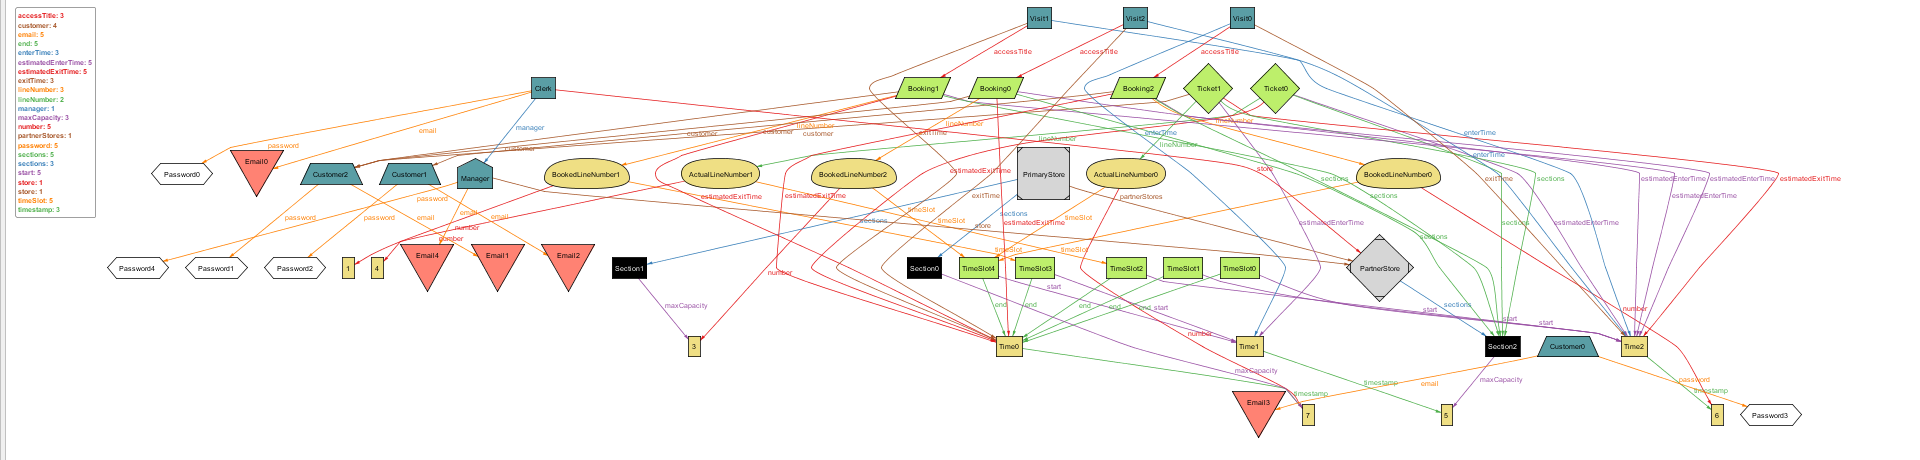
\includegraphics[height=0.7\textwidth]{Images/world1.png}
    \caption{World 1}
\end{figure}

World 1 describes the model in normal conditions, its only purpose is to show an instance of the model without checking
any particular property.

\begin{figure}[H]
    \centering
    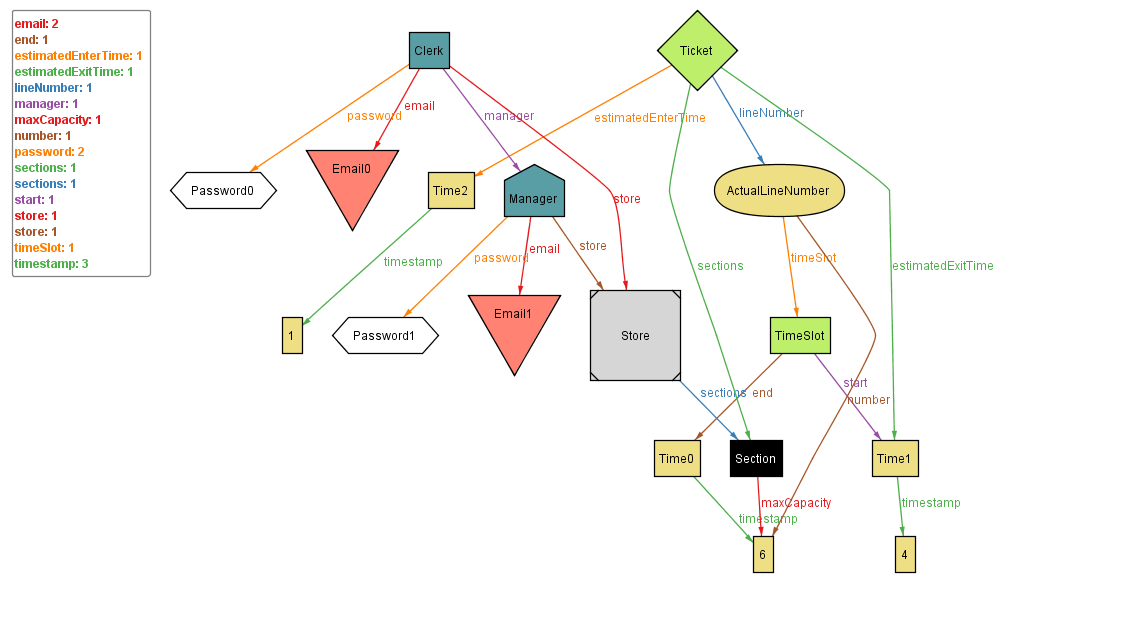
\includegraphics[height=0.5\textwidth]{Images/world2.png}
    \caption{World 2}
\end{figure}

World 2 describes the model when there are no registered customers, so that there can not be bookings and all the
tickets are made as guest going to the clerk in the store.

\begin{figure}[H]
    \centering
    \hspace*{-3.5cm}
    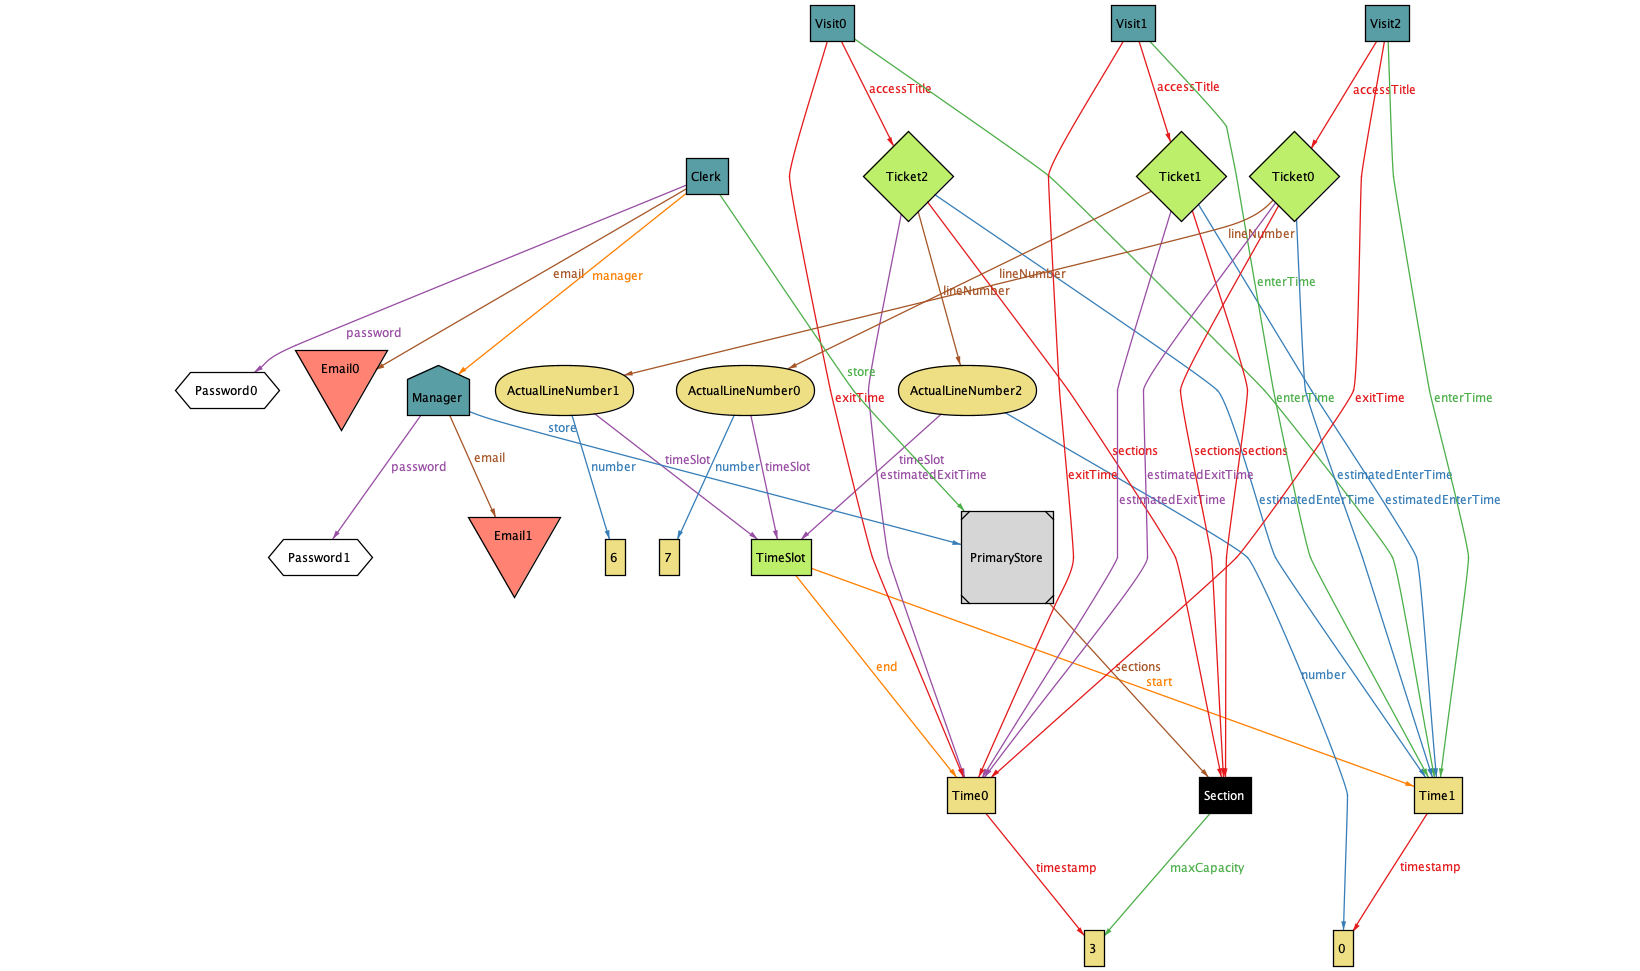
\includegraphics[height=0.7\textwidth]{Images/world3.png}
    \caption{World 3}
\end{figure}

World 3 describes the model when there is only one section and it has the same number of customers as the maximum capacity.

\subsection{Alloy Analyzer results}

6 commands were executed.\\
The results are:\\
\#1: No counterexample found. noMoreVisitsThanAccessTitle may be valid.\\
\#2: No counterexample found. atLeastACustomerForHavingABooking may be valid.\\
\#3: No counterexample found. neverMoreCustomerThanMaxCapacity may be valid.\\
\#4: Instance found.world1 is consistent.\\
\#5: Instance found.world2 is consistent.\\
\#6: Instance found.world3 is consistent.\\


%------------------------------------------------------------------------------------------------------------------------------------------------
\clearpage
{\color{Blue}{\section{Effort Spent}}}
\label{sect:effort}
% Provide here information about how much effort each group member spent in working at this document. We would appreciate details here.
\begin{table}[h]
    \begin{tabular}{|p{2cm}|p{2cm}|p{2cm}|p{1.5cm}|p{8cm}|}
        \hline
        Date:      & Person:       & Part:             & Time (in hours): & Description:                                       \\ \hline
        18/10/2020 & Ozan Incesulu & General Structure & 0.75             & Imported and built the general document structure, switched LF -> CRLF for Windows, replaced template parts with names, year and project title \\ \hline
        18/10/2020 & Ozan Incesulu & Introduction      & 1.5              & Start writing introduction by adding comments for draft goals, adding further subsections, writing basic definition of the system, some abbreviations, definitions, acronyms and references \\ \hline
        24/10/2020 & Ozan Incesulu & Document Structure& 1.5              & Write the document structure of the introduction, provide some comments and assumptions regarding how other parts of the document shall be structured. \\ \hline
        26/10/2020 & Ozan Incesulu & Scope             & 1.25             & Write the Scope section, by defining different users of the system and define different phenomena with the categories they belong. Also add additional definitions. \\ \hline
        26/10/2020 & Aydin Javadov & Scope             & 1                & Extend the goal test to provide details about system function\\ \hline
        29/10/2020 & Ozan Incesulu & Introduction      & 0.25             & Add the clerk role to the system instead of using door automation \\ \hline
        31/10/2020 & Ozan Incesulu & Domain Assumptions& 1                & Write domain assumptions for the system, considering different users and phenomena \\ \hline
        31/10/2020 & Ozan Incesulu & Requirements      & 1.5              & Write system requirements for the system based on agreed goals of the system. \\ \hline
        06/11/2020 & Ozan Incesulu & Goals             & 1                & Write system goals, merge changes from previous team member, some extra housekeeping tasks. \\ \hline
        14/11/2020 & Ozan Incesulu & Use-case          & 1.5              & Export diagrams to images, try to align everything, fix grammar and text \\ \hline
        15/11/2020 & Ozan Incesulu & Product Perspective & 3              & Create state diagrams, write scenarios and explanation \\ \hline
        22/11/2020 & Ozan Incesulu & Product Perspective & 2              & Create class diagram for the system. \\ \hline
        23/11/2020 & Ozan Incesulu & Product Perspective & 1.5            & Add description section, add line number difference to class diagram \\ \hline
        % Line template:
        %          &               &                   &                  &                                                    \\ \hline
    \end{tabular}
\end{table}



%------------------------------------------------------------------------------------------------------------------------------------------------
\clearpage
\nocite{*}
\addcontentsline{toc}{section}{References}
\bibliographystyle{plain}
\bibliography{main}
%------------------------------------------------------------------------------------------------------------------------------------------------




\end{document}
